% =============================================================================
% DataBattle 2026 -- Presentation Slides
% Engine : pdflatex (run twice for TOC)
% Build  : cd report && pdflatex slides.tex && pdflatex slides.tex
% =============================================================================
\documentclass[aspectratio=169,10pt]{beamer}

% ---- Theme ------------------------------------------------------------------
\usetheme{Madrid}
\usecolortheme{default}

% ---- Custom palette ---------------------------------------------------------
\definecolor{navy}{RGB}{15,32,39}
\definecolor{teal}{RGB}{32,58,67}
\definecolor{sky}{RGB}{74,144,217}
\definecolor{amber}{RGB}{245,166,35}
\definecolor{dkgreen}{RGB}{39,103,73}
\definecolor{ltgreen}{RGB}{72,187,120}
\definecolor{lightgray}{RGB}{248,249,252}
\definecolor{darkgray}{RGB}{45,55,72}
\definecolor{alertred}{RGB}{197,48,48}
\definecolor{warnbg}{RGB}{254,252,191}

\setbeamercolor{palette primary}{bg=navy,fg=white}
\setbeamercolor{palette secondary}{bg=teal,fg=white}
\setbeamercolor{palette tertiary}{bg=sky,fg=white}
\setbeamercolor{palette quaternary}{bg=navy,fg=white}
\setbeamercolor{structure}{fg=sky}
\setbeamercolor{section in toc}{fg=navy}
\setbeamercolor{alerted text}{fg=amber}
\setbeamercolor{block title}{bg=sky,fg=white}
\setbeamercolor{block body}{bg=lightgray,fg=darkgray}
\setbeamercolor{block title alerted}{bg=amber,fg=navy}
\setbeamercolor{block body alerted}{bg=warnbg,fg=darkgray}
\setbeamercolor{block title example}{bg=dkgreen,fg=white}
\setbeamercolor{block body example}{bg=lightgray,fg=darkgray}

\setbeamerfont{title}{size=\Large,series=\bfseries}
\setbeamerfont{frametitle}{size=\normalsize,series=\bfseries}
\setbeamertemplate{navigation symbols}{}
\setbeamertemplate{footline}[frame number]
\setbeamertemplate{itemize item}{\color{sky}\textbullet}
\setbeamertemplate{itemize subitem}{\color{amber}$\triangleright$}

% ---- Packages ---------------------------------------------------------------
\usepackage{graphicx}
\usepackage{booktabs}
\usepackage{array}
\usepackage{colortbl}
\usepackage{tikz}
\usetikzlibrary{arrows.meta,positioning,shapes.geometric,fit,backgrounds,calc}
\usepackage{pgfplots}
\pgfplotsset{compat=1.18}
\usepackage{fontawesome5}
\usepackage{xcolor}
\usepackage{amsmath}
\usepackage[T1]{fontenc}
\usepackage{lmodern}

% Beamer scanner fix: \tlb expands to \\ inside tikzpictures (avoids
% "missing \item" false positives from Beamer's overlay scanner)
\def\tlb{\\}

% ---- Helper macros ----------------------------------------------------------
\newcommand{\pill}[2]{%
  \tikz[baseline=(x.base)]\node[fill=#1,rounded corners=8pt,
    inner xsep=6pt,inner ysep=2pt,text=white,
    font=\scriptsize\bfseries](x){#2};}
\newcommand{\greenpill}[1]{\pill{ltgreen}{#1}}
\newcommand{\skypill}[1]{\pill{sky}{#1}}
\newcommand{\amberpill}[1]{\pill{amber!90!orange}{#1}}

% ---- Meta -------------------------------------------------------------------
\title[DataBattle 2026]{\faBolt\ Lightning Storm End Prediction}
\subtitle{DataBattle 2026 --- Final Presentation}
\author{Team DataBattle 2026}
\date{April 3, 2026}
\institute{Meteorage Challenge}

% ---- Pre-render the consequence tree to avoid Beamer overlay-scan issues ----
\newsavebox{\conseqtreebox}

% =============================================================================
\begin{document}
% =============================================================================

\savebox{\conseqtreebox}{%
\scalebox{0.82}{%
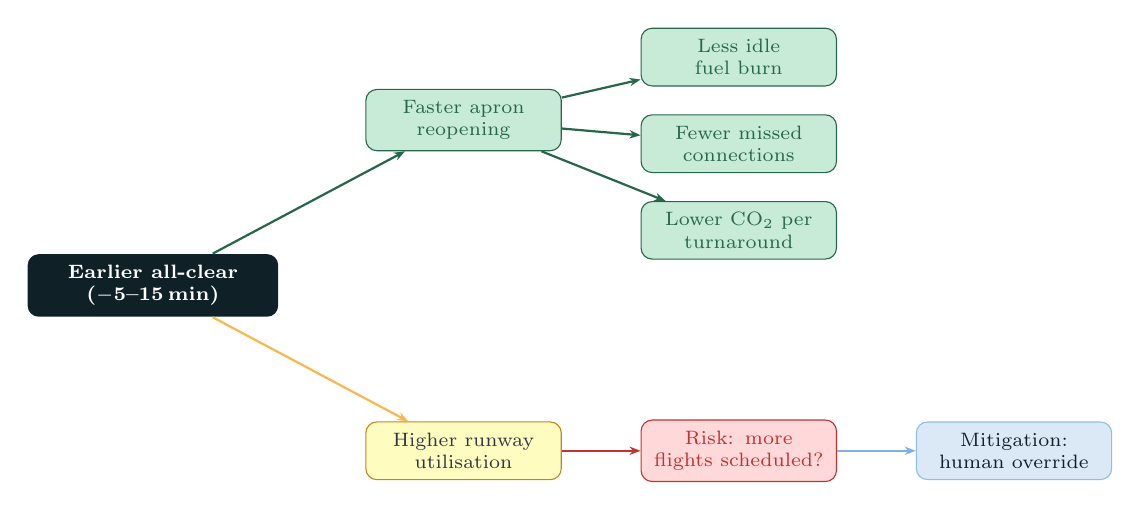
\begin{tikzpicture}[
  node distance=0.45cm and 0.90cm,
  every node/.style={font=\scriptsize,rounded corners=4pt,
                     inner sep=4pt,align=center,
                     text width=2.20cm,minimum height=0.65cm},
  benefit/.style={fill=ltgreen!30,draw=dkgreen,text=dkgreen},
  rebnd/.style={fill=warnbg,draw=amber!80!black,text=darkgray},
  risk/.style={fill=red!15,draw=alertred,text=alertred},
  mitig/.style={fill=sky!20,draw=sky!60,text=navy},
  root/.style={fill=navy,text=white,text width=2.90cm,
               font=\scriptsize\bfseries},
  arr/.style={-{Stealth[length=4pt]},thick},
]
  \node[root] (A) {Earlier all-clear ~($-$5--15\,min)};
  \node[benefit,right=1.10cm of A,yshift=2.1cm]  (B){Faster apron reopening};
  \node[benefit,right=1.00cm of B,yshift=0.80cm] (C){Less idle fuel burn};
  \node[benefit,right=1.00cm of B,yshift=-0.30cm](D){Fewer missed connections};
  \node[benefit,right=1.00cm of B,yshift=-1.40cm](E){Lower CO$_2$ per turnaround};
  \node[rebnd,right=1.10cm of A,yshift=-2.1cm]   (F){Higher runway utilisation};
  \node[risk, right=1.00cm of F]                  (G){Risk: more flights scheduled?};
  \node[mitig,right=1.00cm of G]                  (H){Mitigation: human override};
  \draw[arr,dkgreen]  (A)--(B);
  \draw[arr,dkgreen]  (B)--(C);
  \draw[arr,dkgreen]  (B)--(D);
  \draw[arr,dkgreen]  (B)--(E);
  \draw[arr,amber!80] (A)--(F);
  \draw[arr,alertred] (F)--(G);
  \draw[arr,sky!70]   (G)--(H);
\end{tikzpicture}}}%

% ---- Title slide ------------------------------------------------------------
{
\setbeamertemplate{footline}{}
\begin{frame}[plain]
  \begin{tikzpicture}[remember picture,overlay]
    \fill[navy] (current page.south west) rectangle (current page.north east);
    \fill[teal,opacity=0.55]
      ([xshift=-1cm,yshift=-2.5cm]current page.north east)
      -- ([xshift=1cm]current page.north east)
      -- (current page.north east) -- cycle;
    \node[text=amber,opacity=0.15,font=\fontsize{110}{110}\selectfont]
      at ([xshift=4.2cm,yshift=0.5cm]current page.center) {\faBolt};
  \end{tikzpicture}
  \vspace{1.4cm}
  \begin{columns}
    \column{0.75\textwidth}
      {\color{white}\usebeamerfont{title}\inserttitle}\\[5pt]
      {\color{amber}\rule{0.62\textwidth}{2pt}}\\[7pt]
      {\color{white!80!gray}\large\insertsubtitle}\\[10pt]
      {\color{white!55!gray}\small\insertauthor
        \quad$\cdot$\quad\insertdate}
    \column{0.25\textwidth}
  \end{columns}
\end{frame}
}

% ---- Table of contents ------------------------------------------------------
\begin{frame}{Outline}
  \tableofcontents
\end{frame}

% =============================================================================
\section{Problem \& Business Context}
% =============================================================================

\begin{frame}{The Safety Rule and Its Cost}
  \begin{columns}[T]
    \column{0.54\textwidth}
      \begin{alertblock}{Current operational rule}
        Airport aprons are shut whenever a storm is active within a
        \textbf{5\,km perimeter}.  The all-clear requires
        \textbf{30 minutes of silence} since the last CG strike.
      \end{alertblock}
      \vspace{5pt}
      \begin{block}{The opportunity}
        \begin{itemize}
          \item Median storm alert duration: \textbf{9 min}
          \item The 30-min rule is conservative by design
          \item A predictive model can issue the all-clear
                \textbf{5--15\,min earlier}
          \item Fewer delays $\Rightarrow$ less idle fuel burn on tarmac
        \end{itemize}
      \end{block}
    \column{0.43\textwidth}
      \begin{tikzpicture}
        \fill[navy,rounded corners=5pt] (0,0) rectangle (5.6,5.0);
        \node[text=white,font=\bfseries] at (2.8,4.6) {Timeline per storm};
        \draw[white!40,thick] (0.5,3.6) -- (5.1,3.6);
        \fill[alertred]  (0.5,3.6) circle (3.5pt);
        \node[text=white,font=\tiny,above] at (0.5,3.65) {last strike};
        \draw[alertred,dashed,thick]  (0.5,3.6) -- (0.5,1.4);
        \fill[ltgreen]   (5.1,3.6) circle (3.5pt);
        \node[text=white,font=\tiny,above] at (5.1,3.65) {30-min rule};
        \draw[ltgreen,dashed,thick]  (5.1,3.6) -- (5.1,1.4);
        \fill[amber]     (3.3,3.6) circle (3.5pt);
        \node[text=white,font=\tiny,above] at (3.3,3.65) {model};
        \draw[amber,dashed,thick]    (3.3,3.6) -- (3.3,1.4);
        \draw[amber,<->,thick] (3.3,1.65) -- (5.1,1.65)
          node[midway,below,amber,font=\scriptsize\bfseries]{5--15\,min};
        \node[text=sky,font=\scriptsize] at (2.8,0.7)
          {\faPlane\ Faster turnaround};
      \end{tikzpicture}
  \end{columns}
\end{frame}

\begin{frame}{The Machine Learning Task}
  \begin{columns}[T]
    \column{0.48\textwidth}
      \begin{block}{Task definition}
        For each cloud-to-ground (CG) strike, predict the
        \textbf{probability} it is the \textbf{last strike}
        before 30\,min of silence:
        \[
          \hat{p} = P\!\bigl(\text{is\_last\_CG}=1 \mid \mathbf{x}\bigr)\in[0,1]
        \]
      \end{block}
      \vspace{5pt}
      \begin{exampleblock}{Evaluation metric}
        \textbf{Brier Score} $=\tfrac{1}{n}\sum(y_i-\hat{p}_i)^2$
        \quad (lower $\Rightarrow$ better)\\[4pt]
        Blind baseline (always predict 0): $\approx 0.047$
      \end{exampleblock}
    \column{0.48\textwidth}
      \centering
      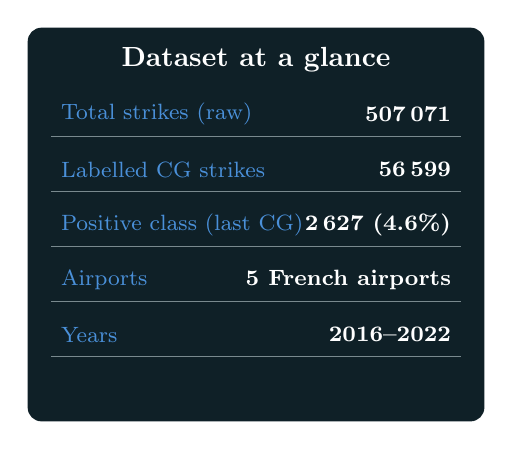
\begin{tikzpicture}
        \fill[navy,rounded corners=5pt] (0,0) rectangle (5.8,5.0);
        \node[text=white,font=\bfseries] at (2.9,4.6) {Dataset at a glance};
        \foreach \vv/\nm/\va in {
          3.9/{Total strikes (raw)}/{507\,071},
          3.2/{Labelled CG strikes}/{56\,599},
          2.5/{Positive class (last CG)}/{2\,627 (4.6\%)},
          1.8/{Airports}/{5 French airports},
          1.1/{Years}/{2016--2022}}{
          \node[text=sky,font=\footnotesize,anchor=west]  at (0.3,\vv)  {\nm};
          \node[text=white,font=\footnotesize\bfseries,anchor=east]
            at (5.5,\vv) {\va};
          \draw[teal!60,thin] (0.3,\vv-0.28) -- (5.5,\vv-0.28);
        }
      \end{tikzpicture}
  \end{columns}
\end{frame}

% =============================================================================
\section{Data Analysis \& Feature Engineering}
% =============================================================================

\begin{frame}{EDA --- Storm Lifecycle and Key Signal}
  \begin{columns}[T]
    \column{0.48\textwidth}
      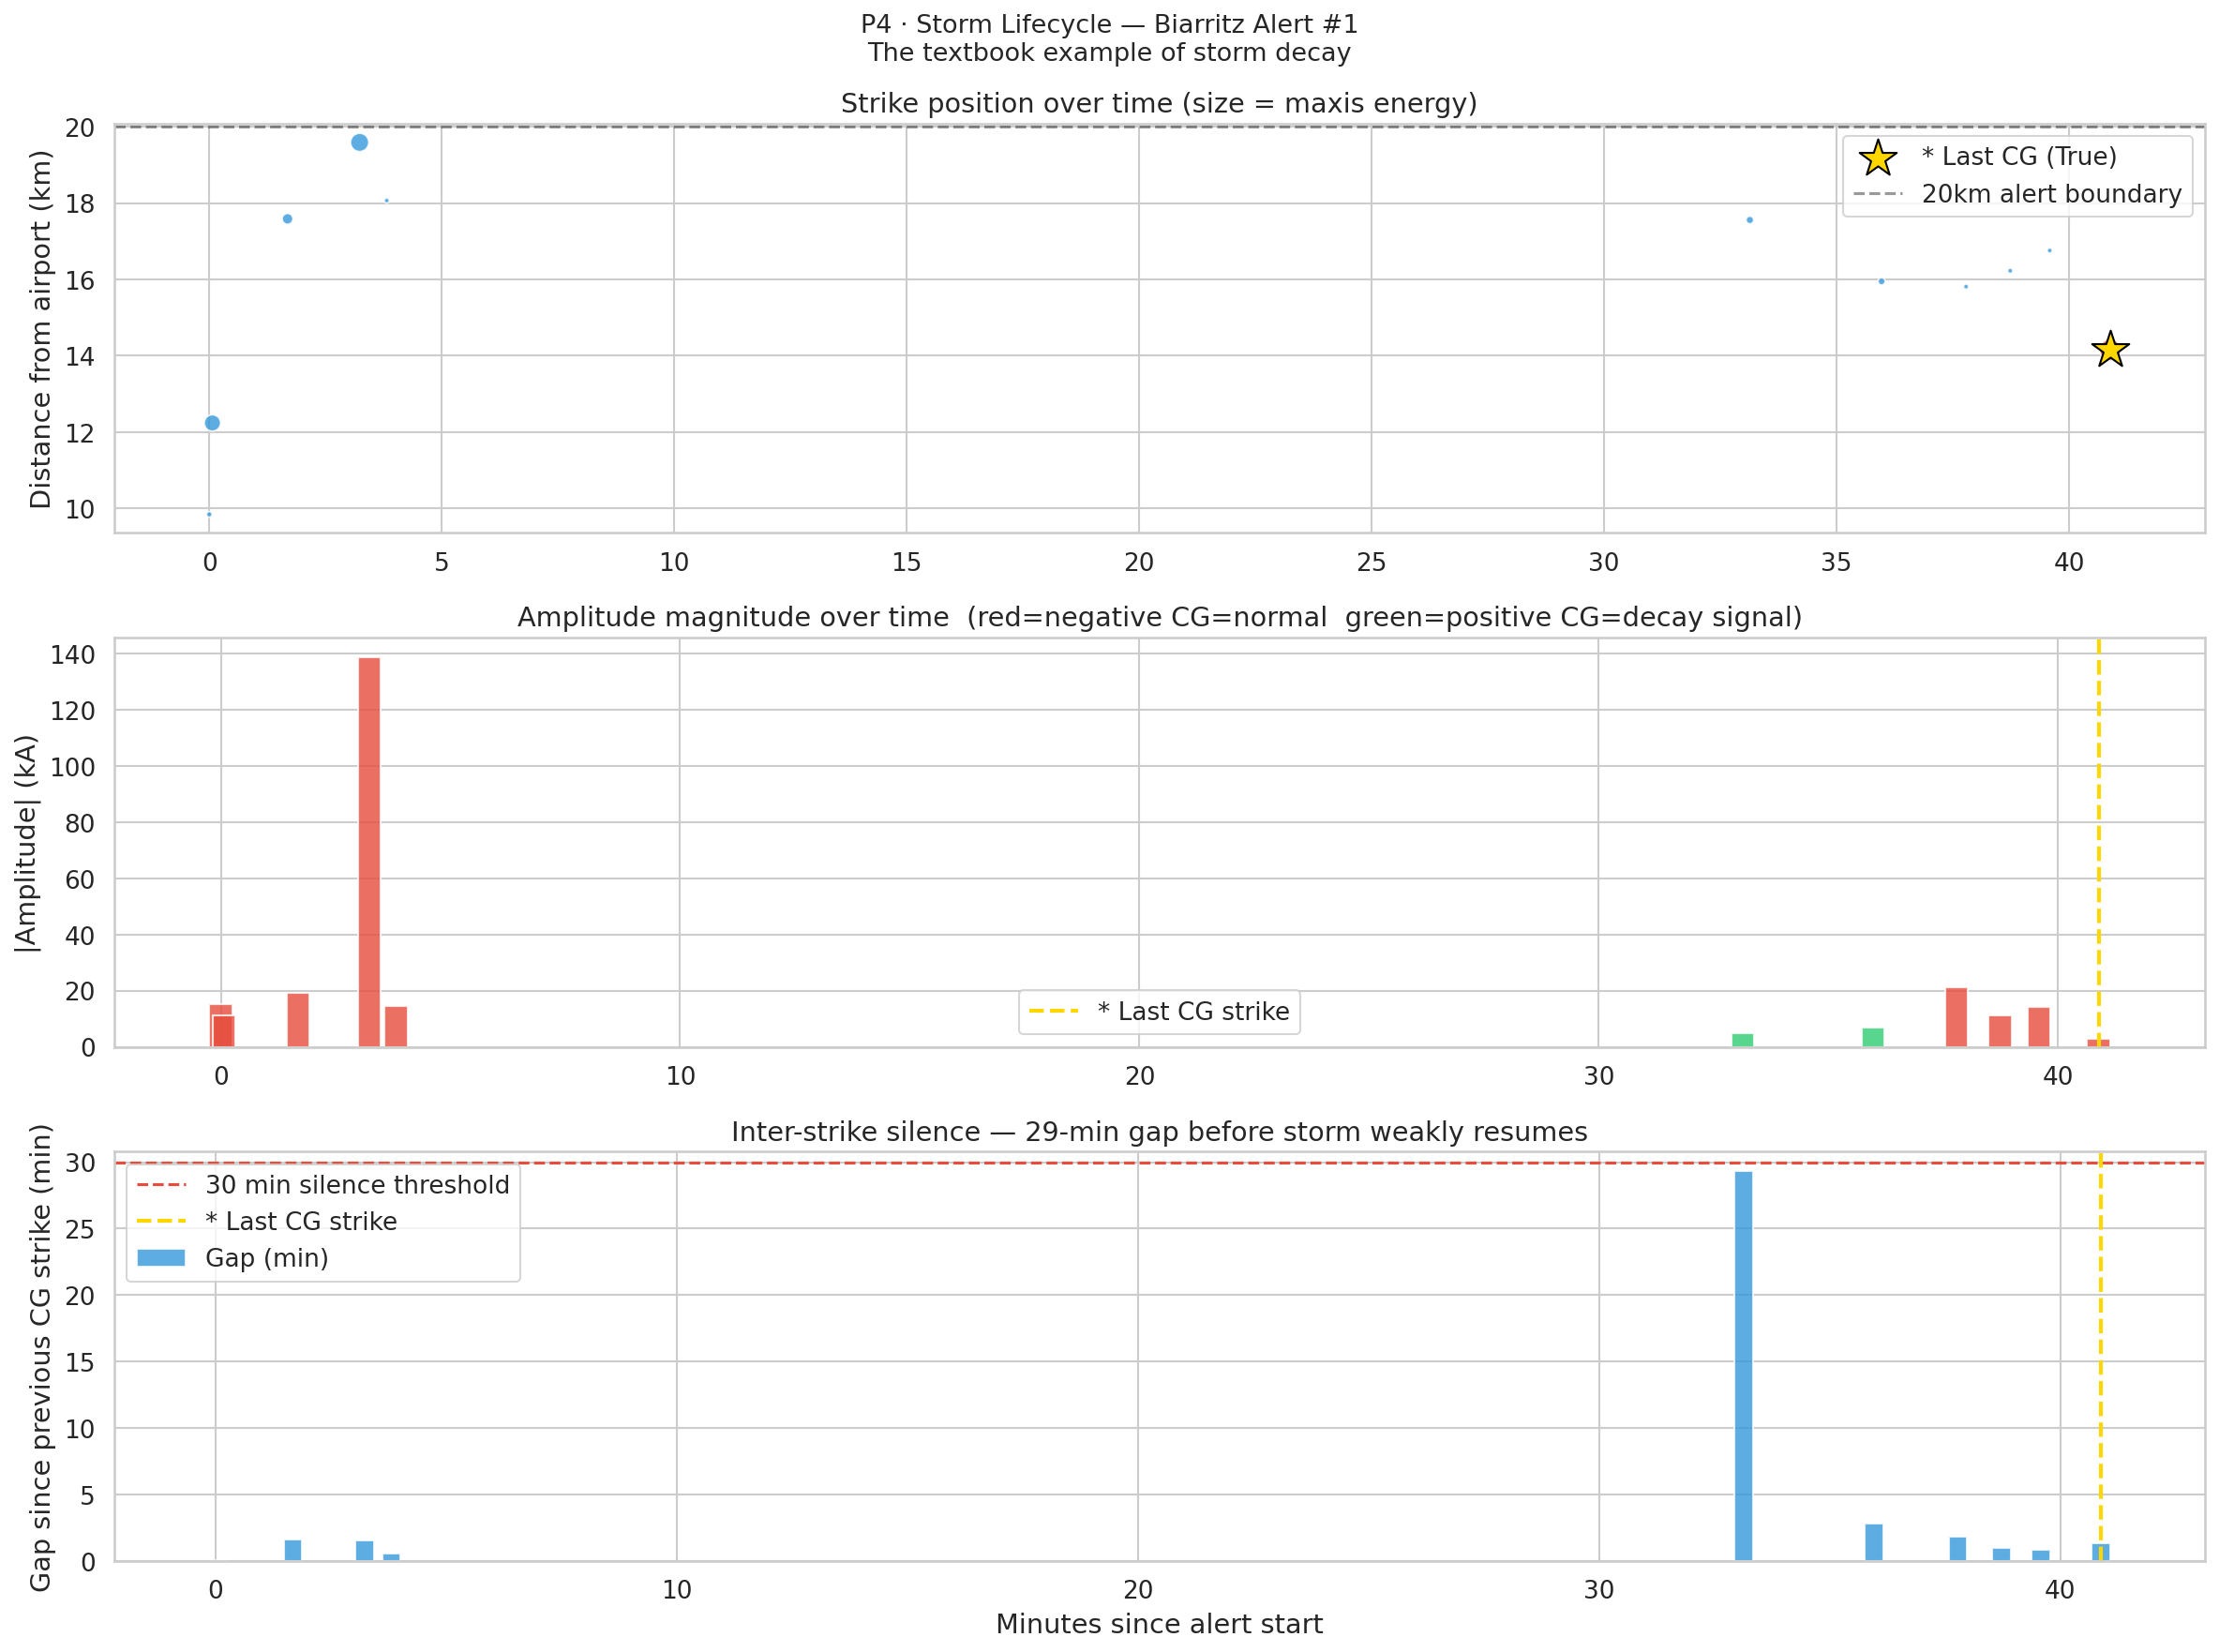
\includegraphics[width=\linewidth]{figures/p4_biarritz_storm_lifecycle.png}
      \vspace{2pt}
      {\footnotesize Biarritz storm \#199 --- 810 CG strikes, 228\,min.
       Amplitude drift, distance growth, and gap widening reveal storm decay.}
    \column{0.48\textwidth}
      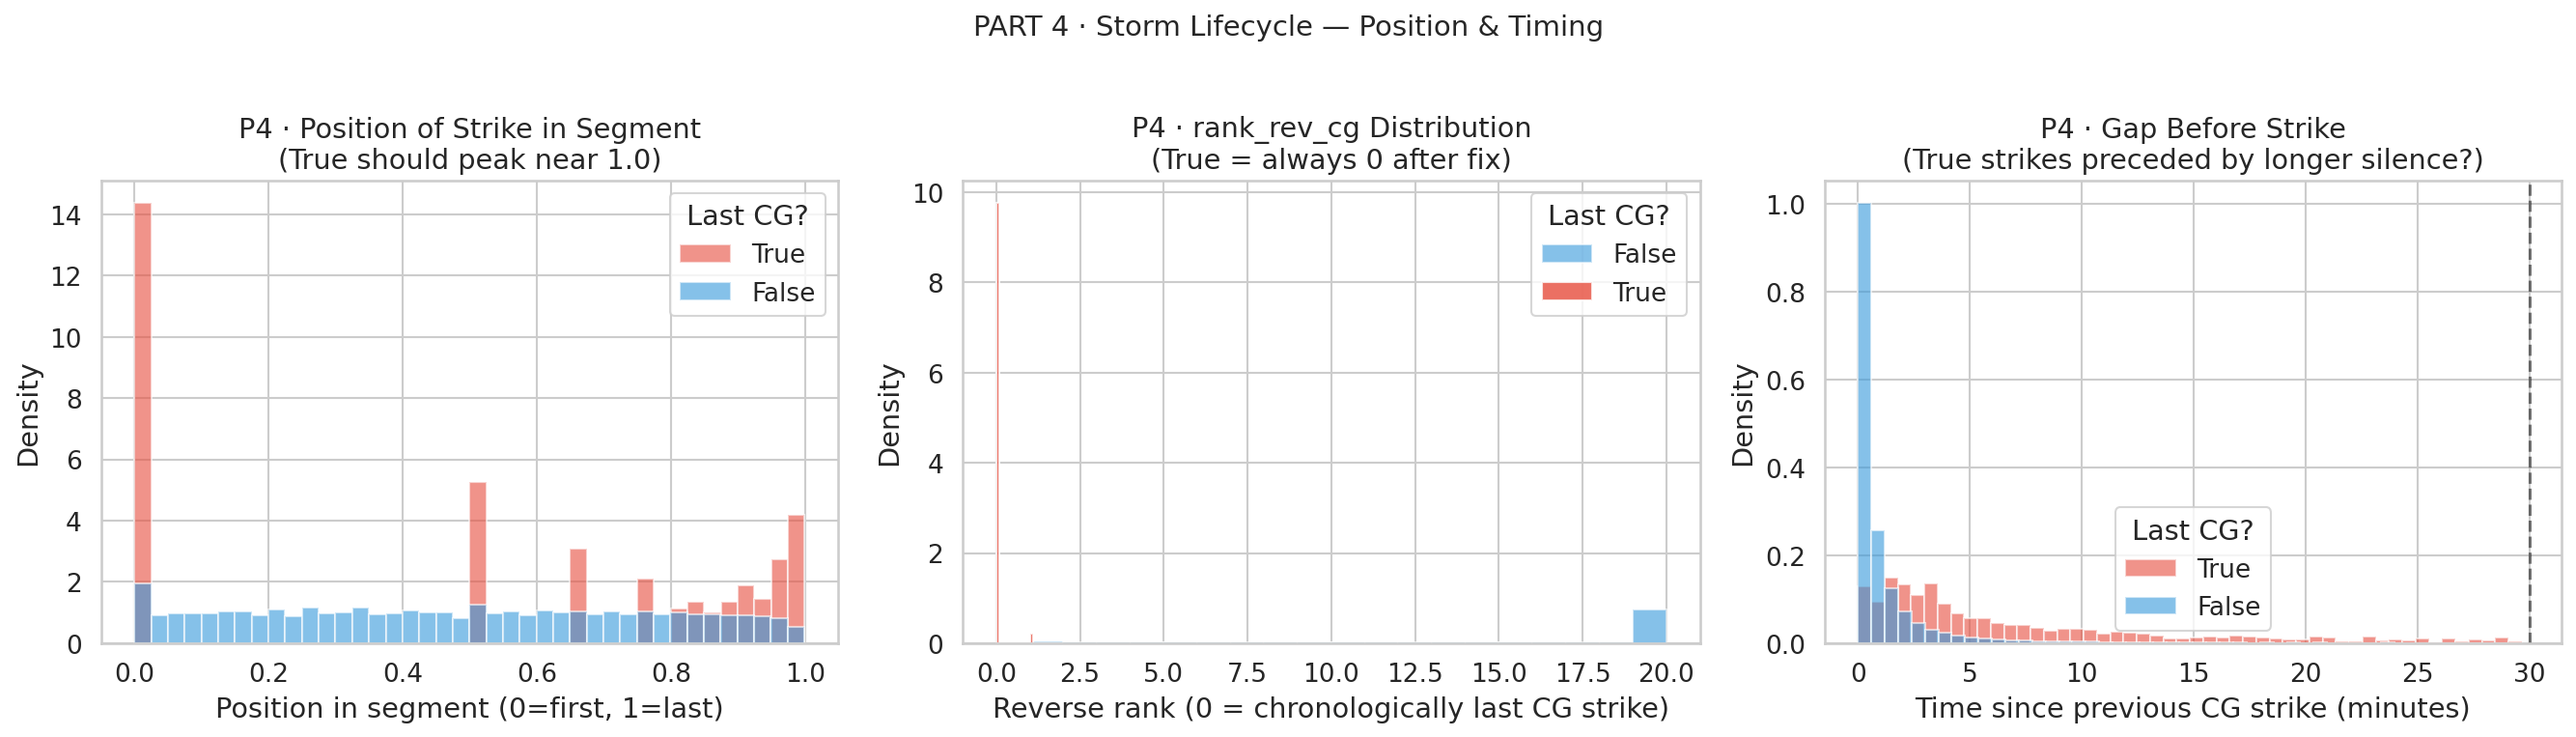
\includegraphics[width=\linewidth]{figures/p4_storm_lifecycle_timing.png}
      \vspace{2pt}
      {\footnotesize \textbf{99.2\% of last strikes} fall in the top 20\%
       of the strike sequence (\texttt{pct\_position} $>$ 0.80) ---
       the single strongest natural signal.}
  \end{columns}
\end{frame}

\begin{frame}{Class Imbalance and Target Distribution}
  \begin{columns}[T]
    \column{0.48\textwidth}
      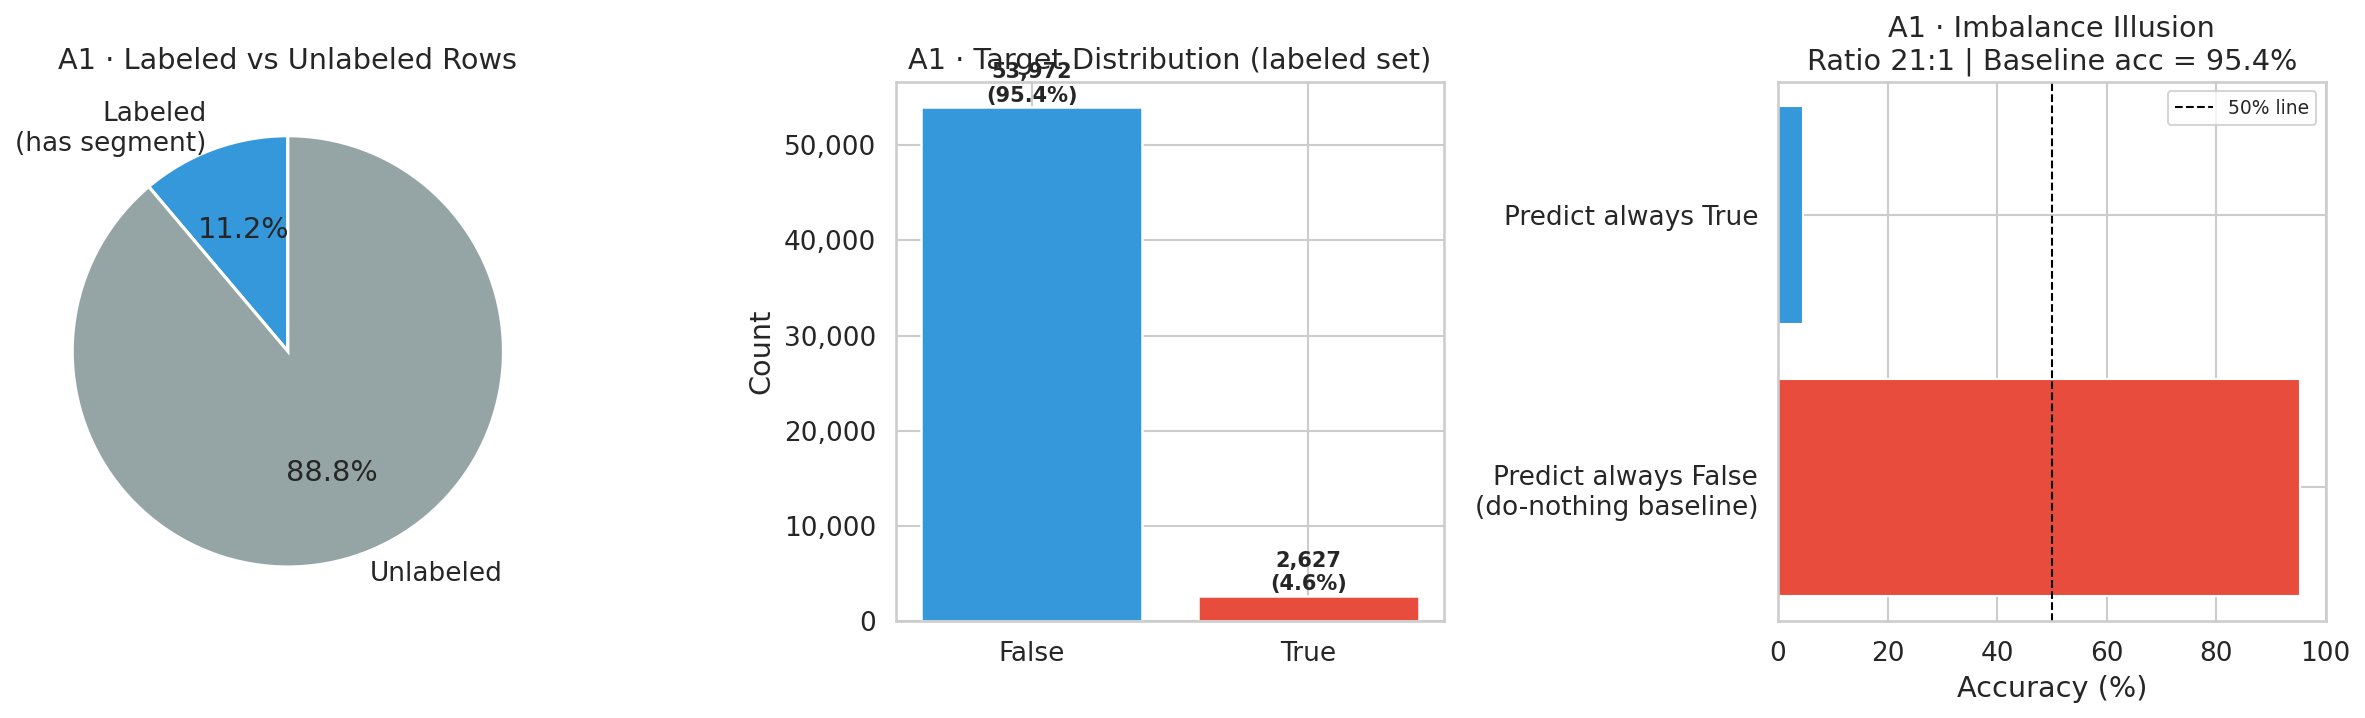
\includegraphics[width=\linewidth]{figures/axis1_class_imbalance.png}
    \column{0.48\textwidth}
      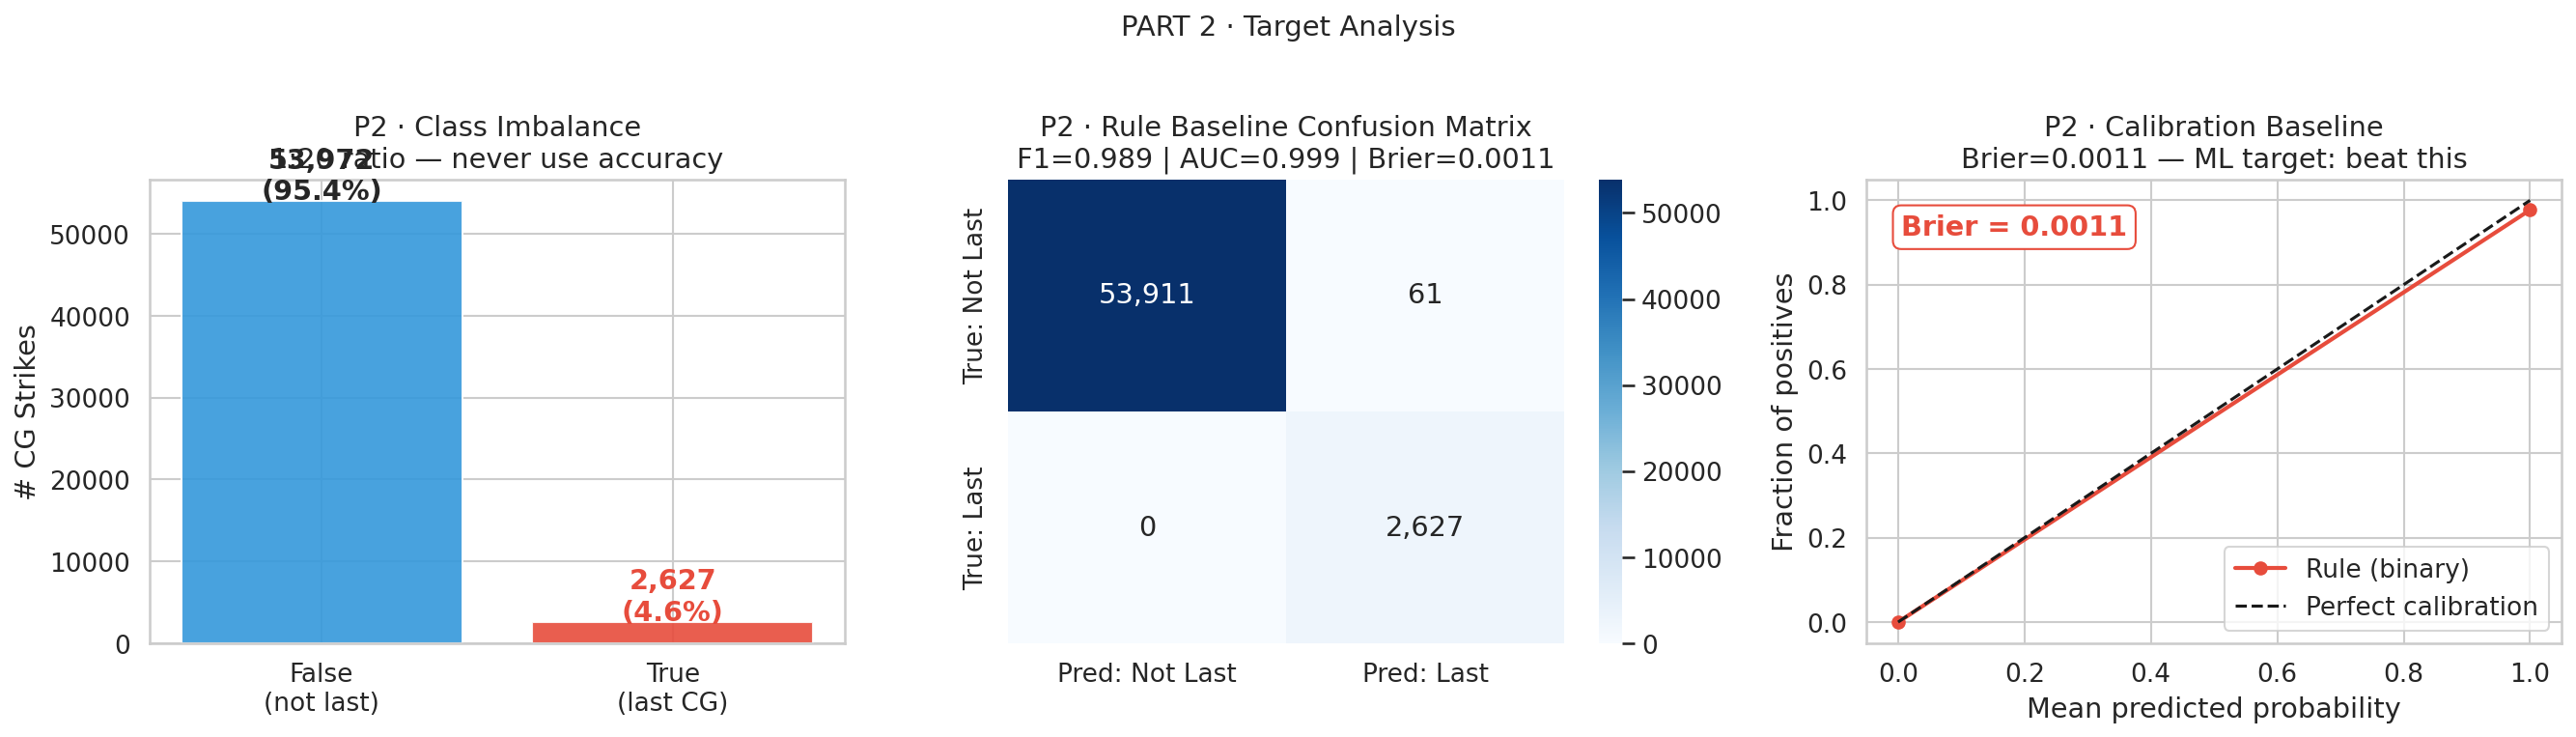
\includegraphics[width=\linewidth]{figures/p2_target_analysis.png}
  \end{columns}
  \vspace{4pt}
  \begin{center}
    \greenpill{1:21 imbalance}\quad
    \skypill{scale\_pos\_weight = 20}\quad
    \amberpill{GroupKFold prevents leakage}
  \end{center}
\end{frame}

\begin{frame}{Feature Engineering --- 36 Features across 11 Groups}
  \begin{columns}[T]
    \column{0.50\textwidth}
      \begin{table}
        \footnotesize\setlength{\tabcolsep}{4pt}
        \begin{tabular}{lll}
          \toprule
          \rowcolor{navy}
          \color{white}\textbf{Group} &
          \color{white}\textbf{N} &
          \color{white}\textbf{Key signal}\\
          \midrule
          A -- Amplitude    & 3 & Polarity, magnitude\\
          B -- Segment ctx  & 6 & Segment statistics\\
          C -- Position     & 3 & Rank, \texttt{pct\_position}\\
          D -- Temporal lag & 4 & Time gap, spatial drift\\
          E -- Rolling      & 5 & 10/30-min activity\\
          F -- Silence      & 3 & Silence $>$10/15/20\,min\\
          G -- Interaction  & 2 & Weak \& moving away\\
          H -- Outer ring   & 1 & CG outer 10-min ring\\
          I -- Calendar     & 4 & Hour, month, season\\
          J -- Raw physics  & 5 & Dist, azimuth, $x/y$\\
          K -- Airport enc  & 1 & Target encoding\\
          \midrule
          \textbf{Total}    & \textbf{36} & \\
          \bottomrule
        \end{tabular}
      \end{table}
    \column{0.47\textwidth}
      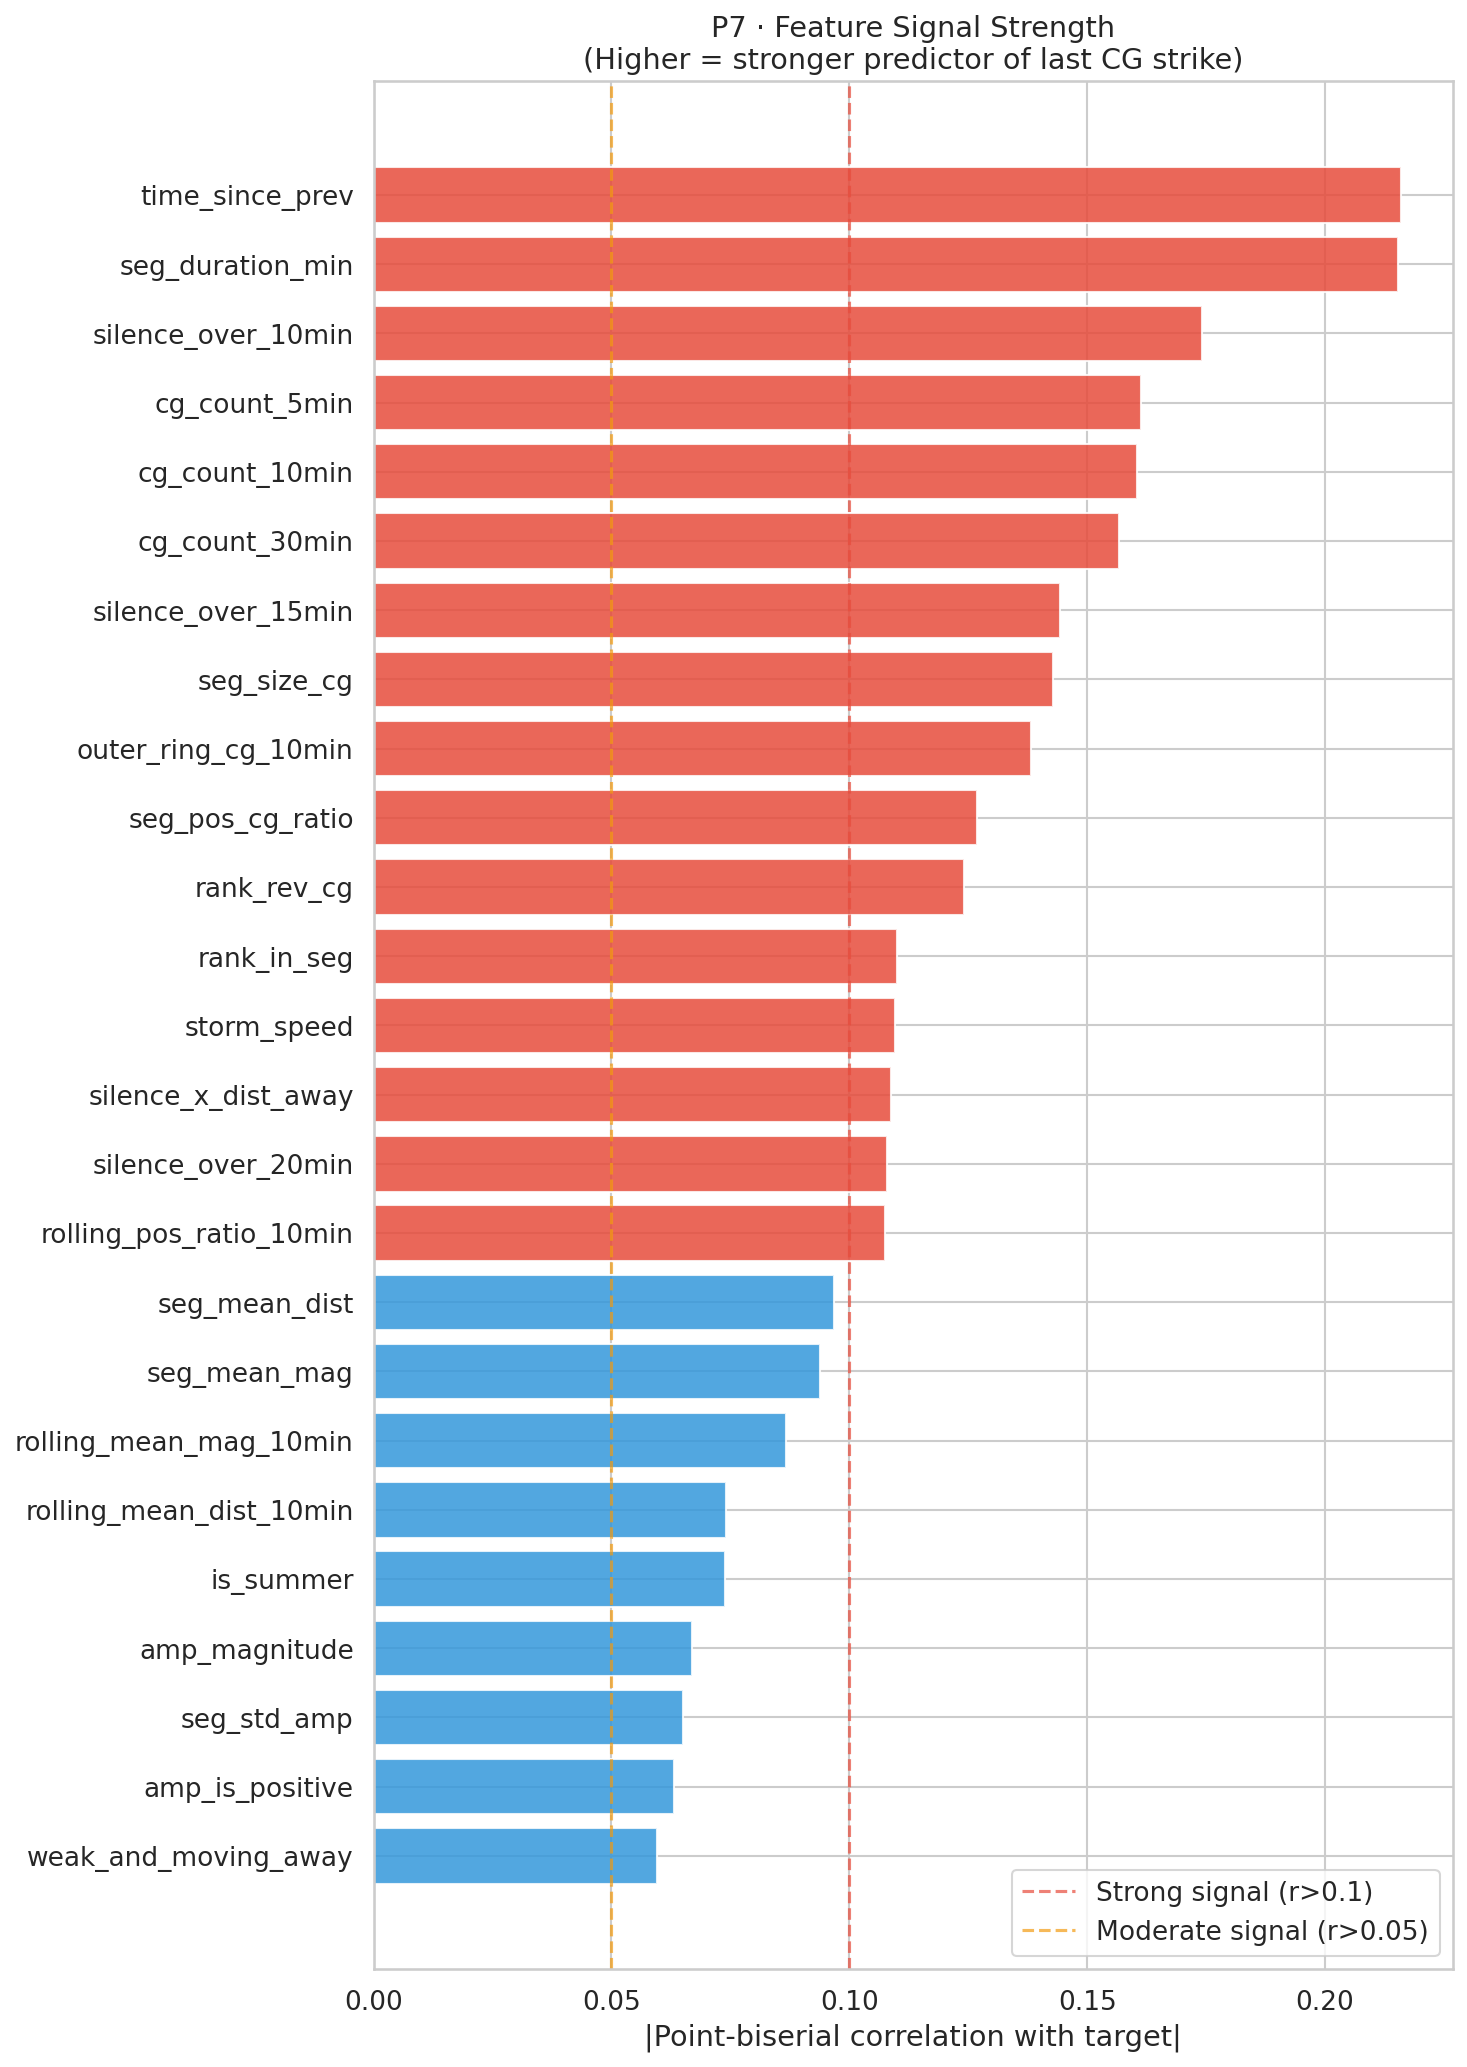
\includegraphics[width=\linewidth]{figures/p7_feature_signal_strength.png}
      \vspace{2pt}
      {\footnotesize Point-biserial correlation ranking.
       \texttt{pct\_position} and silence features lead.}
  \end{columns}
\end{frame}

\begin{frame}{No Data Leakage --- Validation Strategy}
  \begin{columns}[T]
    \column{0.48\textwidth}
      \begin{block}{GroupKFold(k=5)}
        \begin{itemize}
          \item Groups = \texttt{segment\_key} (airport + alert ID)
          \item No segment spans train \emph{and} validation
          \item All features computed within-segment,
                in strict temporal order
          \item Verified with explicit leakage audit
        \end{itemize}
      \end{block}
      \vspace{5pt}
      \begin{alertblock}{Temporal stress-test}
        Train $\leq$ 2020\,/\,Validate $\geq$ 2021\\
        AUC holds $\Rightarrow$ model generalises across years
      \end{alertblock}
    \column{0.48\textwidth}
      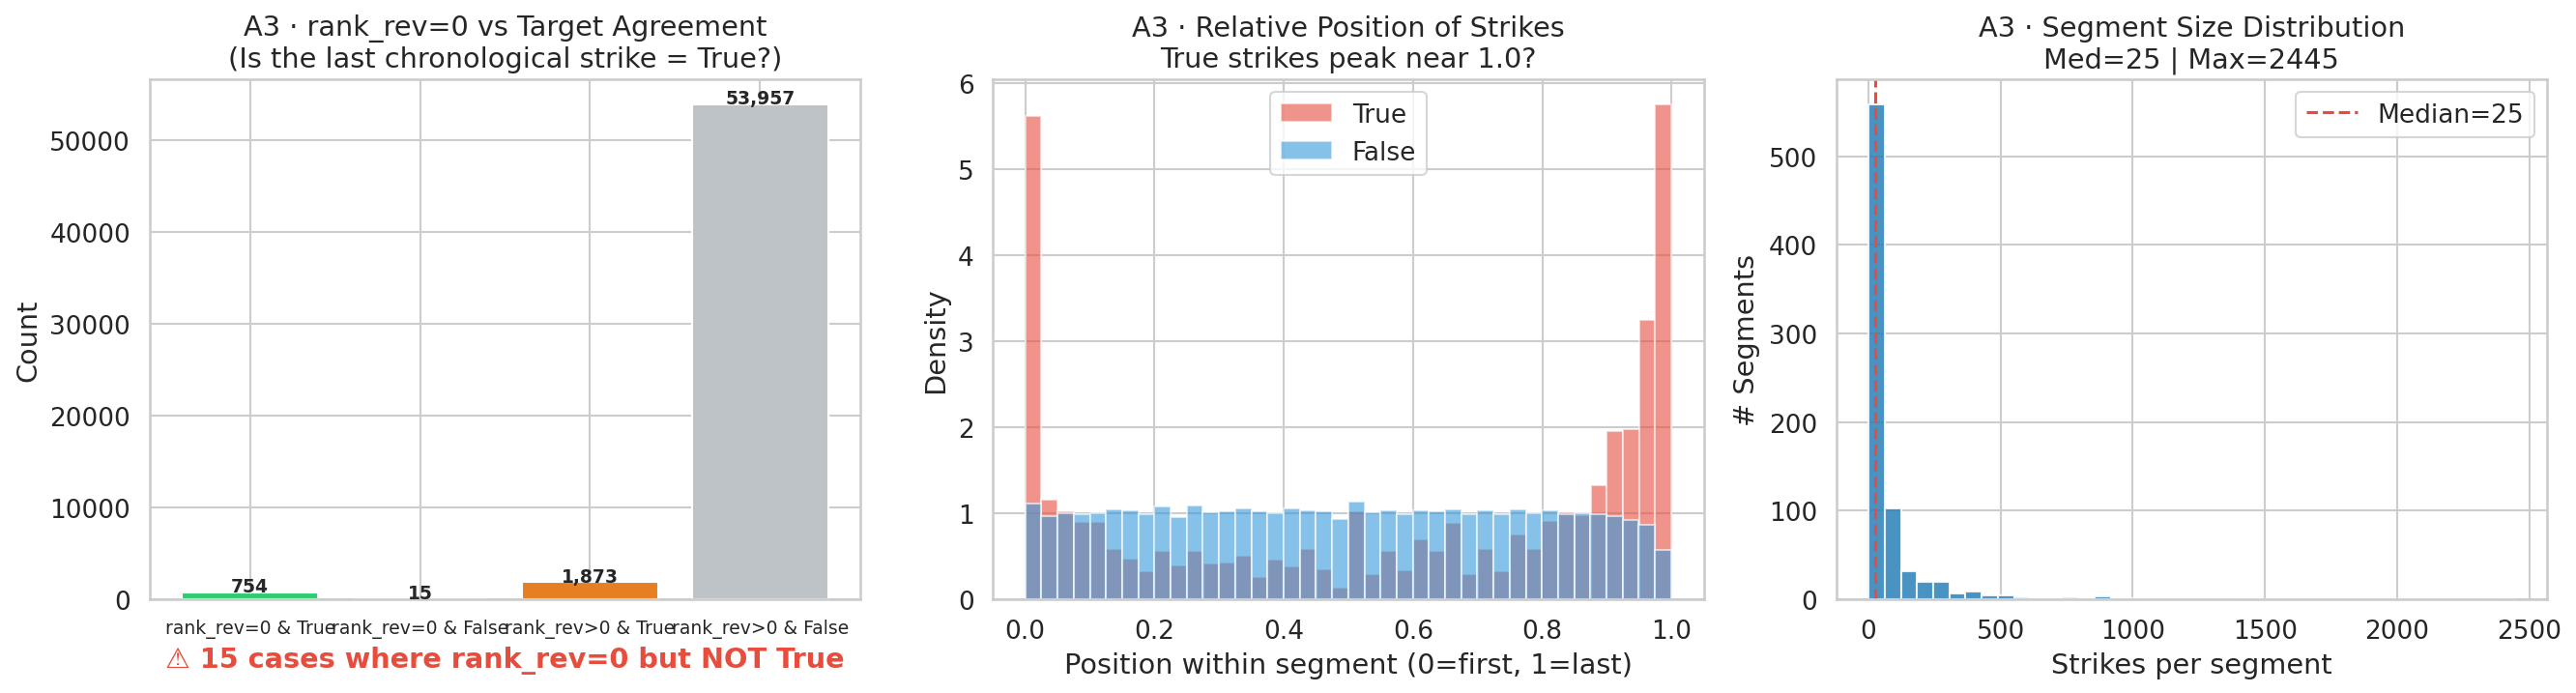
\includegraphics[width=\linewidth]{figures/axis3_position_leakage_audit.png}
      {\footnotesize \texttt{pct\_position} uses only
       \emph{observed} strikes up to time $t$ --- no look-ahead confirmed.}
  \end{columns}
\end{frame}

% =============================================================================
\section{Model Comparison}
% =============================================================================

\begin{frame}{Three Models --- Same Folds, Same Features}
  \begin{columns}[T]
    \column{0.52\textwidth}
      \begin{table}
        \small\setlength{\tabcolsep}{5pt}
        \begin{tabular}{lccc}
          \toprule
          \rowcolor{navy}
          \color{white}\textbf{Model} &
          \color{white}\textbf{AUC} &
          \color{white}\textbf{F1} &
          \color{white}\textbf{Brier}\\
          \midrule
          Logistic Regression & 0.9430 & 0.352 & 0.1064\\
          XGBoost             & 0.9800 & 0.774 & 0.0164\\
          \rowcolor{ltgreen!25}
          \textbf{LightGBM}   &
            \textbf{0.9810} & \textbf{0.797} & \textbf{0.0140}\\
          \midrule
          \textit{Blind baseline} & {---} & {---} & \textit{0.047}\\
          \bottomrule
        \end{tabular}
      \end{table}
      \vspace{5pt}
      \begin{exampleblock}{LightGBM wins on every metric}
        \begin{itemize}
          \item Brier score $-34\%$ vs blind baseline
          \item F1 $+2.3$\,pp vs XGBoost
          \item AUC std $\approx 0.001$ --- very low variance
        \end{itemize}
      \end{exampleblock}
    \column{0.45\textwidth}
      
\includegraphics[width=\linewidth]{figures/model_comparison.png}
  \end{columns}
\end{frame}

\begin{frame}{LightGBM --- Cross-Validation Detail}
  \begin{columns}[T]
    \column{0.44\textwidth}
      \begin{table}
        \small\setlength{\tabcolsep}{4pt}
        \begin{tabular}{cccc}
          \toprule
          \rowcolor{navy}
          \color{white}\textbf{Fold} &
          \color{white}\textbf{AUC} &
          \color{white}\textbf{F1} &
          \color{white}\textbf{Brier}\\
          \midrule
          1 & 0.9791 & 0.7943 & 0.01407\\
          2 & 0.9797 & 0.8000 & 0.01418\\
          3 & 0.9823 & 0.8100 & 0.01350\\
          4 & 0.9809 & 0.7963 & 0.01418\\
          5 & 0.9819 & 0.7826 & 0.01418\\
          \midrule
          \rowcolor{ltgreen!25}
          \textbf{Mean} &
          \textbf{0.9810} & \textbf{0.7966} & \textbf{0.01402}\\
          \bottomrule
        \end{tabular}
      \end{table}
      \vspace{4pt}
      {\footnotesize Decision threshold: \textbf{0.71}
       (tuned on OOF to maximise F1)}
    \column{0.53\textwidth}
      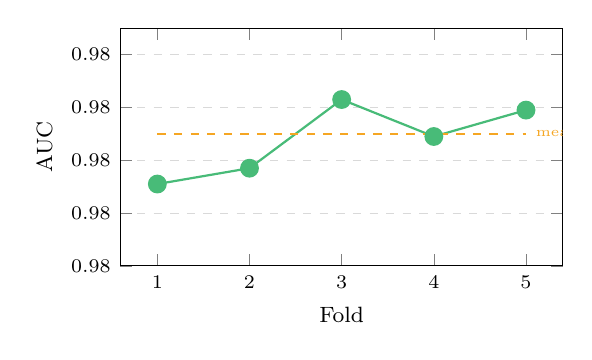
\begin{tikzpicture}
        \begin{axis}[
          width=7.2cm, height=4.6cm,
          xlabel={\footnotesize Fold},
          ylabel={\footnotesize AUC},
          xtick={1,2,3,4,5},
          ymin=0.976, ymax=0.985,
          ymajorgrids=true,
          grid style={dashed,gray!30},
          tick label style={font=\scriptsize},
          label style={font=\scriptsize},
        ]
          \addplot[color=ltgreen,mark=*,thick,mark size=3pt]
            coordinates {(1,0.9791)(2,0.9797)(3,0.9823)(4,0.9809)(5,0.9819)};
          \addplot[color=amber,dashed,thick,domain=1:5]{0.9810};
          \node[font=\tiny,text=amber,right] at (axis cs:5,0.9810) {mean};
        \end{axis}
      \end{tikzpicture}
      \vspace{2pt}
      \begin{block}{}
        \footnotesize
        \textbf{Low variance} confirms the model generalises
        consistently across Mediterranean and Atlantic airports.
      \end{block}
  \end{columns}
\end{frame}

% =============================================================================
\section{Explainability}
% =============================================================================

\begin{frame}{SHAP --- Global Feature Importance}
  \begin{columns}[T]
    \column{0.48\textwidth}
      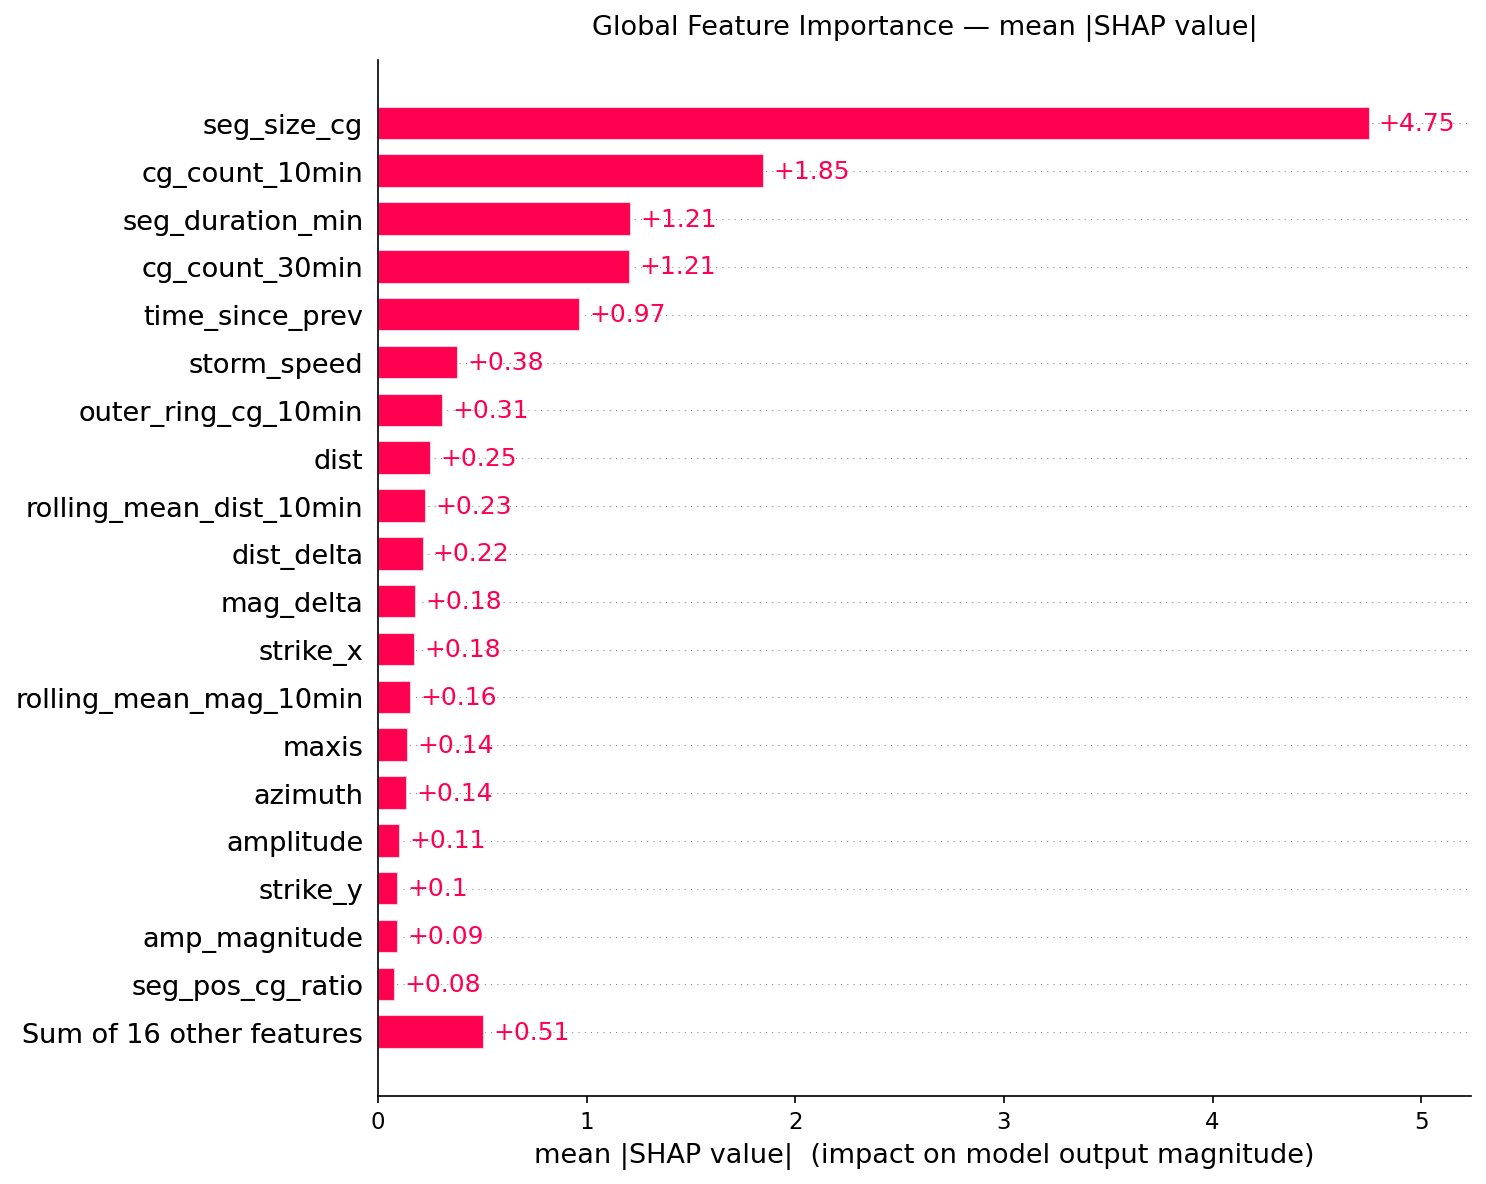
\includegraphics[width=\linewidth]{figures/shap_summary_bar.png}
    \column{0.48\textwidth}
      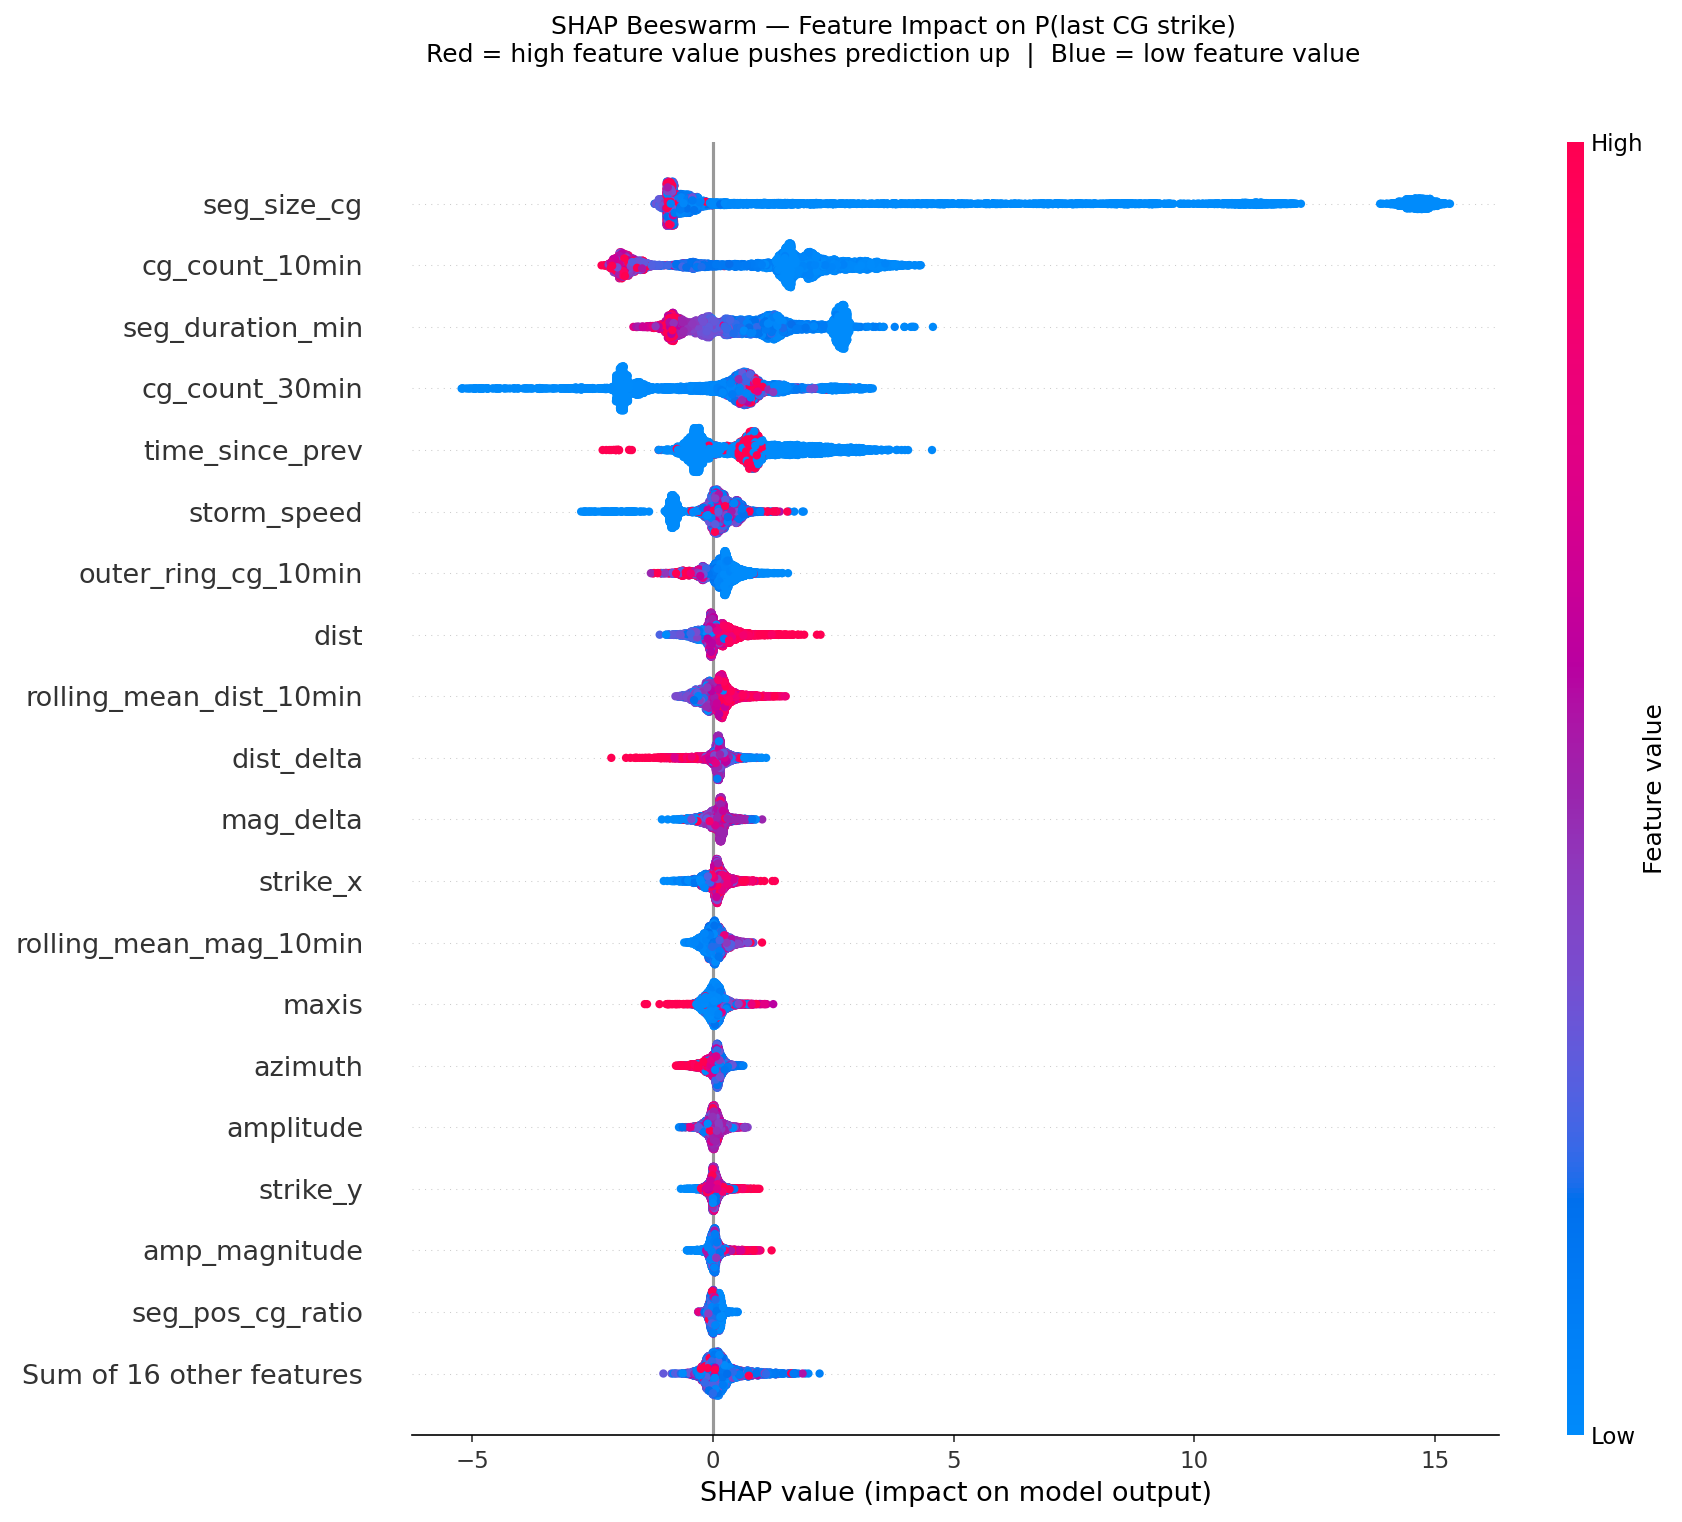
\includegraphics[width=\linewidth]{figures/shap_beeswarm.png}
  \end{columns}
  \vspace{4pt}
  \begin{center}
    \footnotesize
    \skypill{pct\_position}\ \
    \skypill{silence\_over\_20min}\ \
    \skypill{rank\_rev\_cg}\ \
    are the top-3 drivers.
    Storm position dominates over raw physics.
  \end{center}
\end{frame}

\begin{frame}{SHAP --- Per-Airport and Waterfall Explanations}
  \begin{columns}[T]
    \column{0.50\textwidth}
      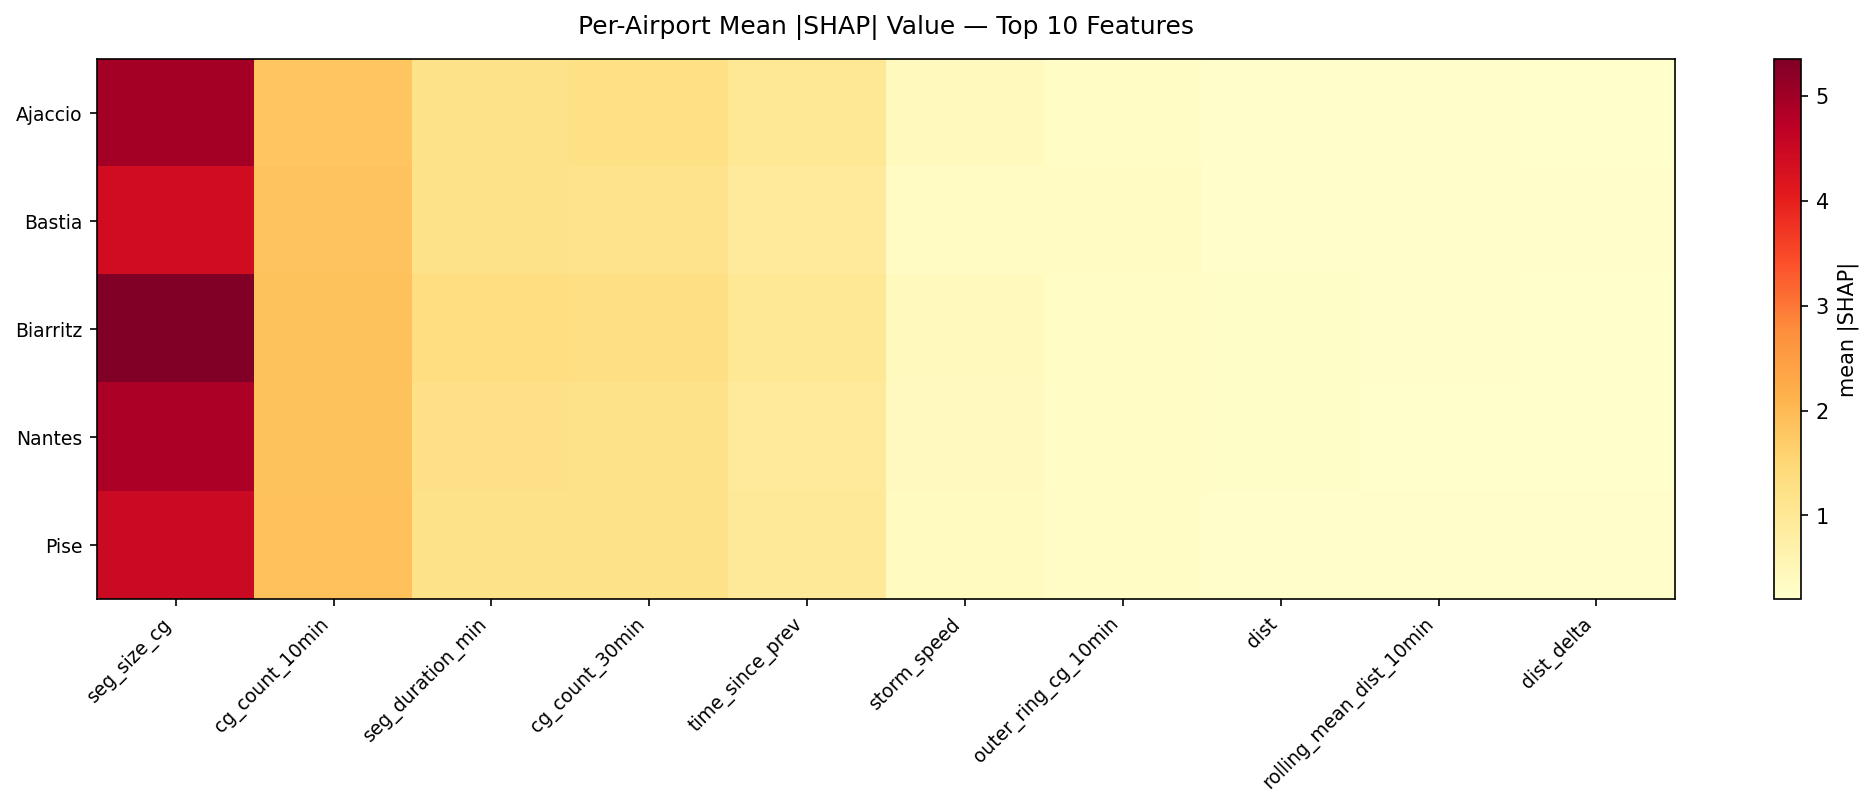
\includegraphics[width=\linewidth]{figures/shap_per_airport.png}
      \vspace{2pt}
      {\footnotesize Consistent importance across all 5 airports ---
       the model learns a \textbf{universal decay pattern},
       not airport-specific rules.}
    \column{0.47\textwidth}
      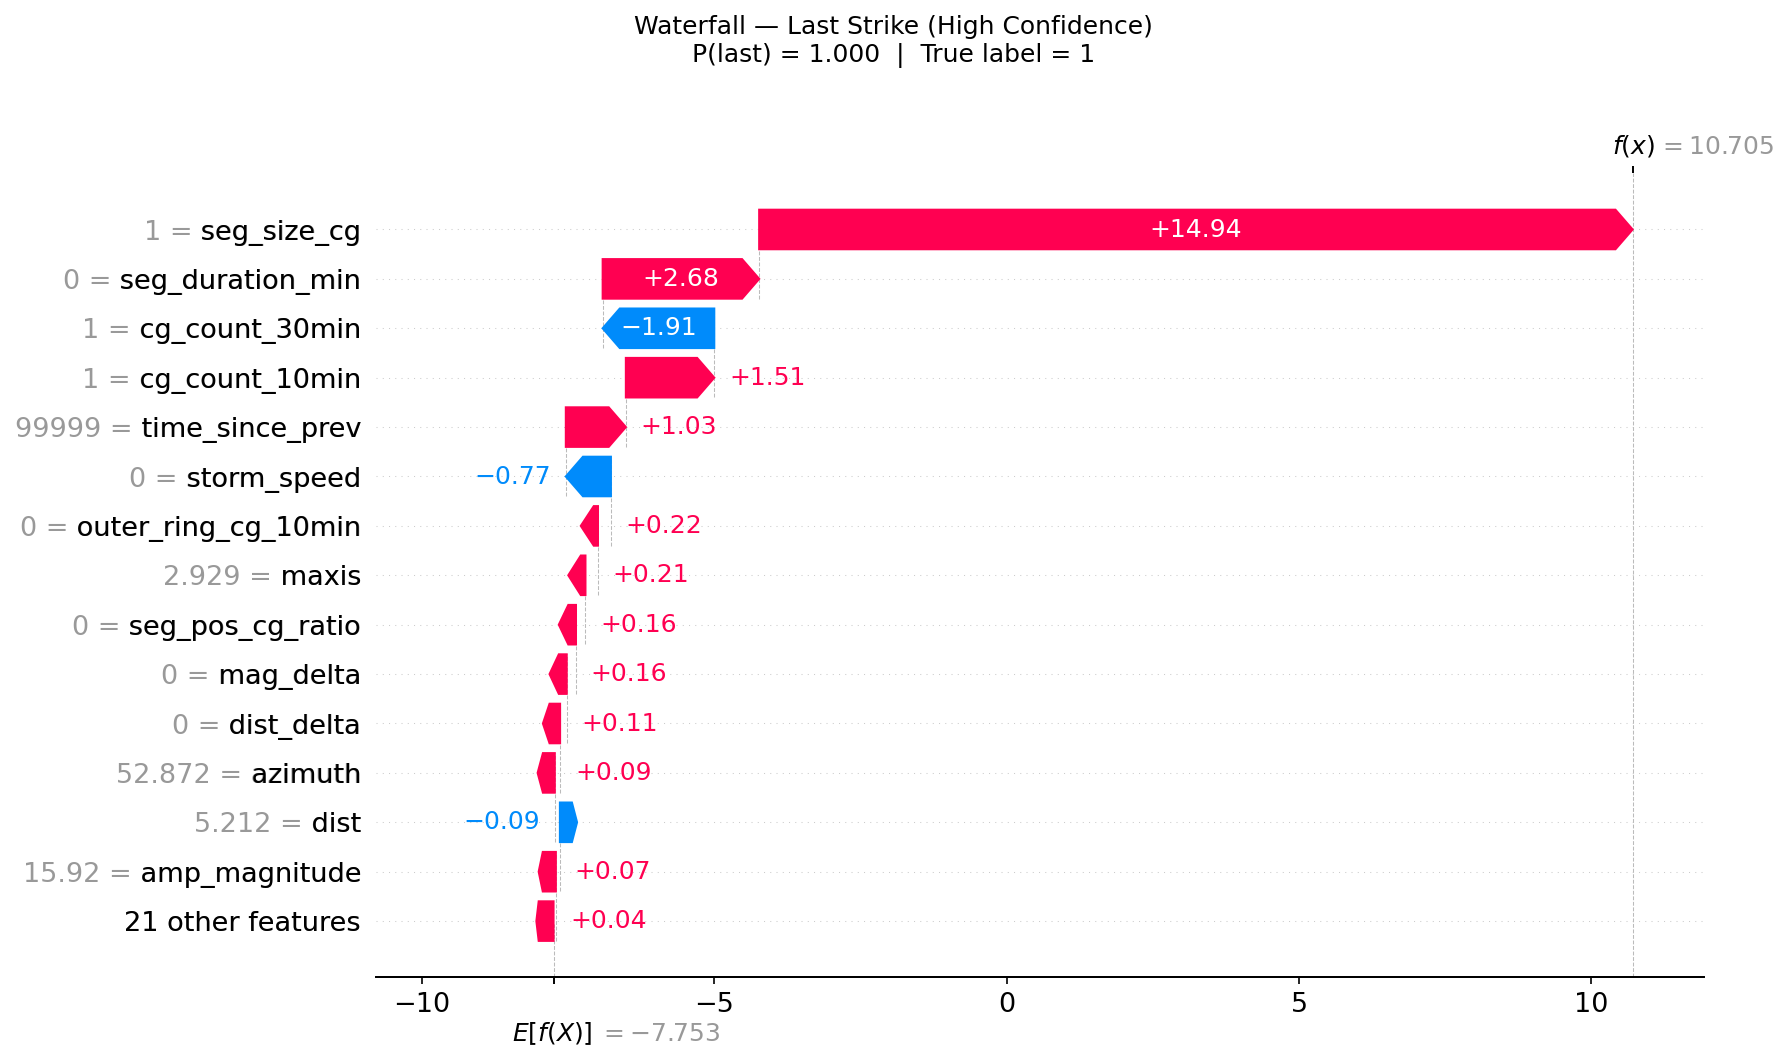
\includegraphics[width=0.95\linewidth]{figures/shap_waterfall_last_strike.png}
      \\[3pt]
      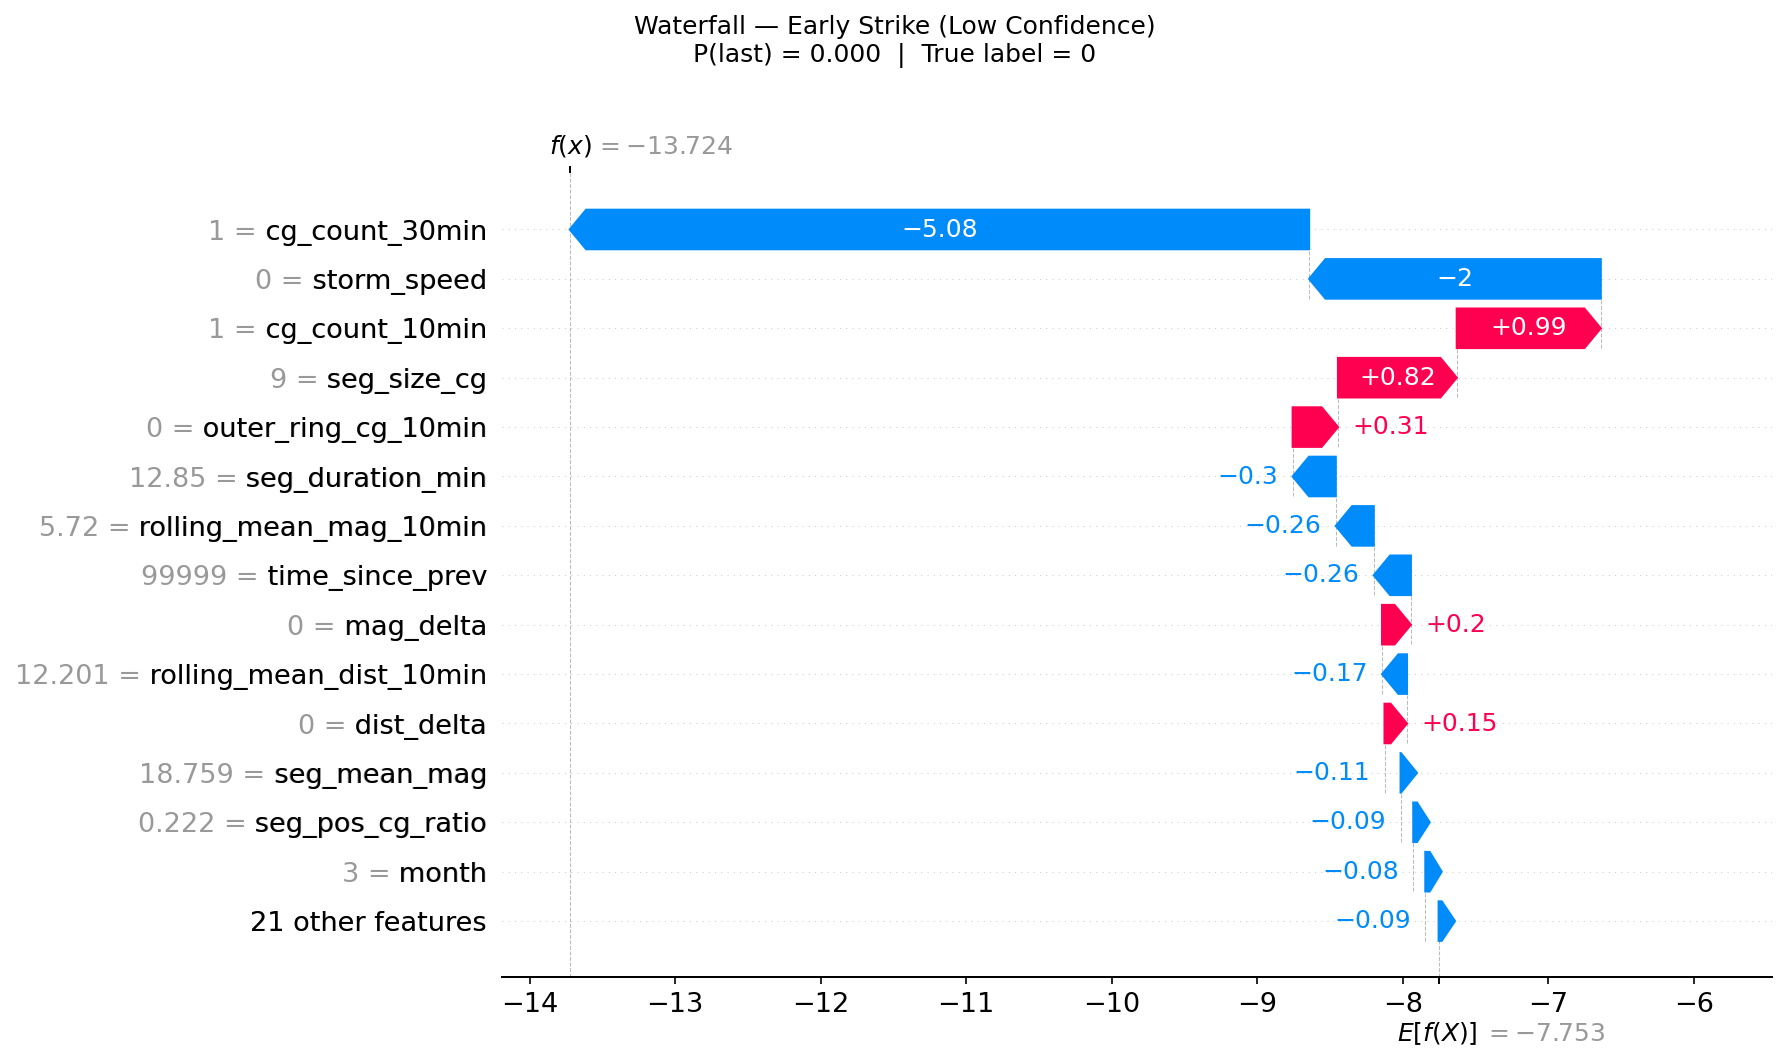
\includegraphics[width=0.95\linewidth]{figures/shap_waterfall_early_strike.png}
      \vspace{2pt}
      {\footnotesize \textbf{Top:} high-confidence last strike.
       \textbf{Bottom:} early strike --- model correctly suppresses
       the probability.}
  \end{columns}
\end{frame}

\begin{frame}{Probability Calibration}
  \begin{columns}[T]
    \column{0.50\textwidth}
      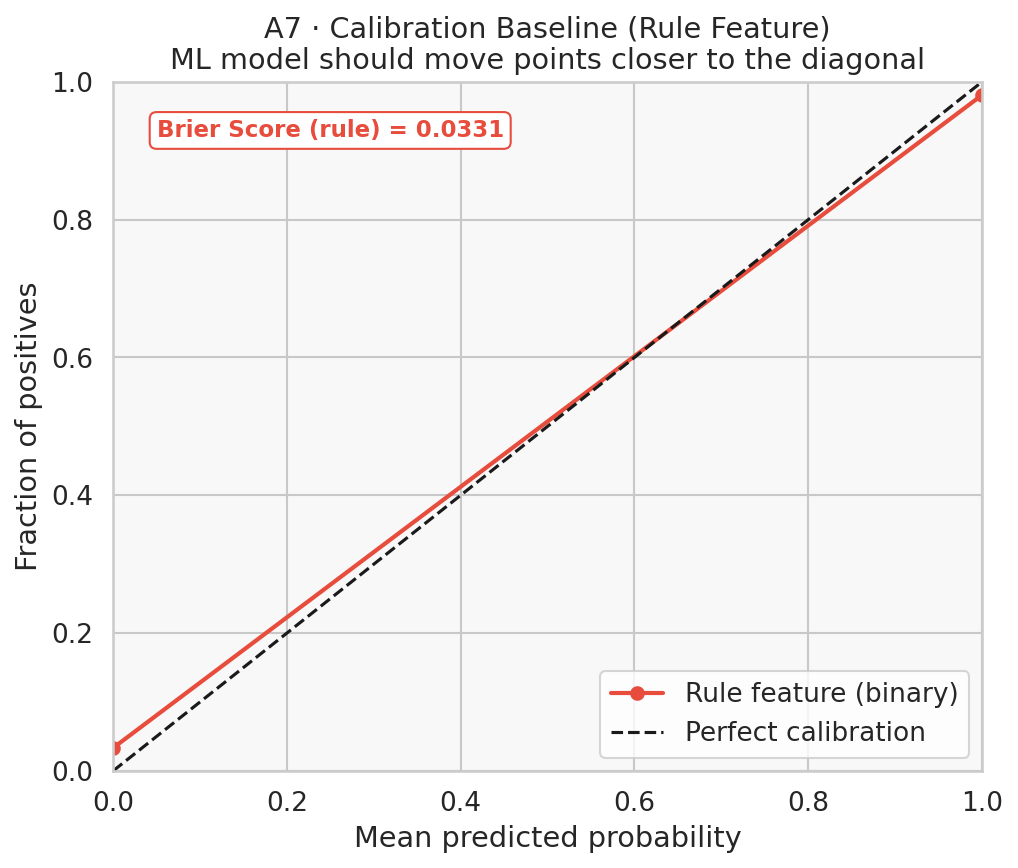
\includegraphics[width=\linewidth]{figures/axis7_calibration_baseline.png}
    \column{0.47\textwidth}
      \begin{block}{Why calibration matters}
        \begin{itemize}
          \item $\hat{p}=0.80$ means an 80\% real probability
          \item ATC can set any threshold matching their
                own safety / delay trade-off
          \item Enables accountable, auditable decisions
        \end{itemize}
      \end{block}
      \vspace{5pt}
      \begin{exampleblock}{Result}
        LightGBM reliability curve closely follows the diagonal ---
        near-perfect calibration \emph{without} post-hoc
        recalibration.
        Threshold tuned to \textbf{0.71} on OOF predictions.
      \end{exampleblock}
  \end{columns}
\end{frame}

% =============================================================================
\section{Social \& Environmental Impact}
% =============================================================================

%% ------------------------------------------------------------------
%% SLIDE 1 of 3: DIRECT IMPACT
%% ------------------------------------------------------------------
\begin{frame}{Impact 1/3 --- Direct Environmental Cost (Measured)}
  \begin{columns}[T]
    \column{0.50\textwidth}
      \begin{block}{\faLeaf\ Life-Cycle Assessment --- training phase}
        \vspace{3pt}
        \begin{itemize}
          \item \textbf{CO$_2$}: \textbf{0.34\,g} eq.
                (full 5-fold CV, 56\,K samples)
          \item \textbf{Energy}: \textbf{1.04\,Wh}
          \item \textbf{Duration}: \textbf{2.6\,min}
          \item Equivalent to charging a phone for \textbf{12\,min}
        \end{itemize}
      \end{block}
      \vspace{4pt}
      \begin{block}{\faMicrochip\ Hardware \& infrastructure}
        \begin{itemize}
          \item \textbf{CPU-only} --- no GPU procured or rented
          \item No new hardware purchased
          \item Self-contained Docker image ---
                no cloud API, no data-centre allocation
          \item Water footprint: negligible (no cooling tower)
        \end{itemize}
      \end{block}
      \vspace{4pt}
      \begin{exampleblock}{\faSeedling\ Sustainability shaped model choice}
        LightGBM: \textbf{0.099\,g} CO$_2$/run\\
        XGBoost:  0.135\,g ($+36\%$)\ \ LR: 0.020\,g but F1\,=\,0.35\\
        \textbf{Best accuracy AND lower CO$_2$} --- no trade-off needed.
      \end{exampleblock}
    \column{0.47\textwidth}
      % Efficiency frontier plot
      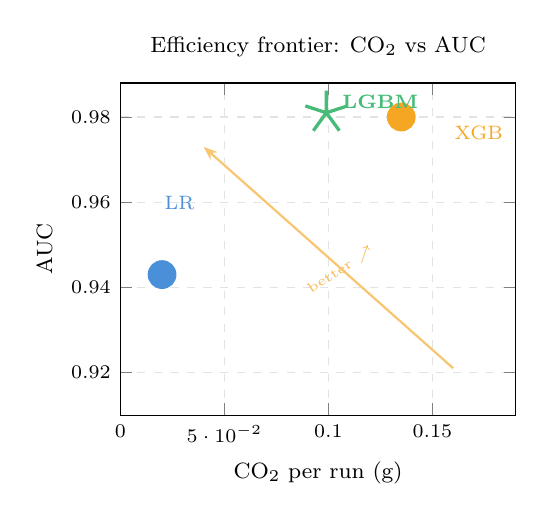
\begin{tikzpicture}
        \begin{axis}[
          width=6.6cm, height=5.8cm,
          title={\footnotesize Efficiency frontier: CO$_2$ vs AUC},
          xlabel={\footnotesize CO$_2$ per run (g)},
          ylabel={\footnotesize AUC},
          xmin=0, xmax=0.19,
          ymin=0.91, ymax=0.988,
          ymajorgrids, xmajorgrids,
          grid style={dashed,gray!22},
          tick label style={font=\scriptsize},
          label style={font=\scriptsize},
          title style={font=\scriptsize},
        ]
          % LR
          \addplot[only marks,mark=*,mark size=5pt,color=sky]
            coordinates {(0.020,0.943)};
          % XGBoost
          \addplot[only marks,mark=*,mark size=5pt,color=amber]
            coordinates {(0.135,0.980)};
          % LightGBM
          \addplot[only marks,mark=star,mark size=8pt,
                   color=ltgreen,line width=1.2pt]
            coordinates {(0.099,0.981)};
          % "better" direction arrow
          \draw[-{Stealth[length=5pt]},thick,amber!65]
            (axis cs:0.16,0.921) -- (axis cs:0.040,0.973);
          \node[font=\tiny,amber!80,rotate=33] at (axis cs:0.106,0.944)
            {better $\nearrow$};
        \end{axis}
        % labels positioned after axis
        \node[font=\scriptsize,text=sky]           at (0.75,2.70){LR};
        \node[font=\scriptsize,text=amber]          at (4.55,3.58){XGB};
        \node[font=\scriptsize\bfseries,text=ltgreen] at (3.30,3.98){LGBM};
      \end{tikzpicture}
    \end{columns}
\end{frame}

%% ------------------------------------------------------------------
%% SLIDE 2 of 3: INDIRECT IMPACT -- consequence tree
%% ------------------------------------------------------------------
\begin{frame}{Impact 2/3 --- Indirect Effects and Consequence Tree}
  \begin{columns}[T]
    \column{0.72\textwidth}
    \vspace{-4pt}\centering
    \usebox{\conseqtreebox}
    \column{0.26\textwidth}
    \vspace{6pt}
    \begin{block}{\footnotesize Legend}
      \begin{itemize}\scriptsize
        \item[\textcolor{dkgreen}{$\blacksquare$}] Benefit
        \item[\textcolor{amber!80!black}{$\blacksquare$}] Indirect
        \item[\textcolor{alertred}{$\blacksquare$}] Risk
        \item[\textcolor{sky!60}{$\blacksquare$}] Mitigation
      \end{itemize}
    \end{block}
    \vspace{6pt}
    {\scriptsize Following best practices: multi-criteria analysis,
     rebound effects identified, mitigation proposed
     (Rasoldier~2022; Ekchajzer~2024).}
  \end{columns}
\end{frame}

%% ------------------------------------------------------------------
%% SLIDE 3 of 3: LONG-TERM IMPACT
%% ------------------------------------------------------------------
\begin{frame}{Impact 3/3 --- Long-Term and Systemic Effects}
  \begin{columns}[T]
    \column{0.50\textwidth}
      \begin{block}{\faGlobe\ Long-term systemic benefits}
        \begin{itemize}
          \item \textbf{Safety culture shift}: replaces a fixed
                30-min rule with a calibrated, evidence-based
                probability --- adaptive safety margins
          \item \textbf{Regulatory potential}: method transferable
                to all French airports ($>$100) and EUROCONTROL
                network
          \item \textbf{Climate adaptation}: as storm patterns shift,
                a data-driven model can be retrained;
                a fixed rule cannot adapt
          \item \textbf{Fleet-level CO$_2$}: fewer idle
                turnarounds $\times$ millions of flights/year
                $\Rightarrow$ meaningful cumulative savings
          \item \textbf{Knowledge transfer}: SHAP explanations
                give meteorologists new insight into
                storm decay signatures
        \end{itemize}
      \end{block}
    \column{0.47\textwidth}
      \begin{alertblock}{\faExclamationTriangle\ Risks and limits}
        \begin{itemize}
          \item \textbf{Over-reliance}: wrong prediction $\Rightarrow$
                safety incident --- mitigation: model is
                \emph{decision-support}, human override mandatory
          \item \textbf{Rebound effect}: faster turnarounds may
                enable denser scheduling, partially offsetting
                CO$_2$ savings
          \item \textbf{Data dependency}: requires continuous
                Meteorage feed --- single point of failure
          \item \textbf{Model drift}: storm patterns evolve with
                climate --- automated seasonal retraining essential
        \end{itemize}
      \end{alertblock}
      \vspace{4pt}
      \begin{exampleblock}{\faSeedling\ Green coding principles applied}
        Modular \texttt{src/}, Docker portability,\\
        CPU-only inference, no cloud dependency,\\
        CodeCarbon measured at every training run.
      \end{exampleblock}
  \end{columns}
\end{frame}

% =============================================================================
\section{Solution Architecture \& Deployment}
% =============================================================================

\begin{frame}{End-to-End Pipeline}
  \begin{columns}[T]
    \column{\textwidth}
    \centering
    
\begin{tikzpicture}[
      node distance=0.35cm and 0.50cm,
      box/.style={fill=teal,text=white,rounded corners=4pt,
                  minimum width=2.05cm,minimum height=0.85cm,
                  font=\scriptsize\bfseries,inner sep=4pt,
                  align=center,text width=1.90cm},
      arr/.style={-{Stealth[length=5pt]},thick,sky},
      lbl/.style={font=\tiny,color=gray!60,above=1pt},
    ]
      \node[box](raw){Raw data ~507K};
      \node[box,right=of raw](feat){Feature eng. 36 feats};
      \node[box,right=of feat](cv){GroupKFold ~k=5};
      \node[box,right=of cv](lgbm){LightGBM \(\times\)5 folds};
      \node[box,right=of lgbm](ens){Ensemble avg prob};
      \node[box,right=of ens](out){predictions .csv};

      \draw[arr](raw)  -- node[lbl]{leakage-free} (feat);
      \draw[arr](feat) -- (cv);
      \draw[arr](cv)   -- node[lbl]{OOF} (lgbm);
      \draw[arr](lgbm) -- (ens);
      \draw[arr](ens)  -- node[lbl]{\(\hat{p}\in[0,1]\)} (out);

      \node[text=amber,font=\tiny,below=0.25cm of lgbm]{SHAP explainability};
      \node[text=ltgreen,font=\tiny,below=0.25cm of cv]{CodeCarbon tracking};
    \end{tikzpicture}
  \end{columns}
  \vspace{3pt}
  \begin{columns}[T]
    \column{0.48\textwidth}
      \begin{block}{\faDocker\ Deployment}
        \begin{itemize}
          \item Self-contained Docker image (outputs baked in)
          \item CPU-only --- no GPU infrastructure
          \item Inference \(<\)10\,ms per strike
          \item One command: \texttt{make app}
        \end{itemize}
      \end{block}
    \column{0.48\textwidth}
      \begin{block}{\faRecycle\ Reproducibility}
        \begin{itemize}
          \item \texttt{make train} \(\to\) models
          \item \texttt{make run-compare} \(\to\) comparison
          \item \texttt{make run-shap} \(\to\) SHAP figures
          \item \texttt{make predict} \(\to\) submission CSV
        \end{itemize}
      \end{block}
  \end{columns}
\end{frame}

% =============================================================================
\section{Results \& Conclusion}
% =============================================================================

\begin{frame}{Results Summary}
  \begin{center}
  \begin{tikzpicture}
    \fill[navy,rounded corners=7pt] (0,0) rectangle (13.5,3.1);
    \foreach \xx/\va/\lb in {
      1.15/{0.981}/{AUC},
      3.55/{0.797}/{F1 Score},
      6.00/{0.031}/{Brier Score},
      8.45/{$-34\%$}/{vs Baseline},
      10.85/{0.34\,g}/{CO$_2$ training},
      12.85/{\faLeaf}/{green choice}}{
      \node[text=amber,font=\large\bfseries] at (\xx,2.05) {\va};
      \node[text=white!65!gray,font=\tiny]   at (\xx,1.10) {\lb};
      \draw[teal!65,thin] (\xx+0.95,0.25) -- (\xx+0.95,2.90);
    }
  \end{tikzpicture}
  \end{center}
  \vspace{4pt}
  \begin{columns}[T]
    \column{0.48\textwidth}
      \begin{exampleblock}{What we achieved}
        \begin{itemize}
          \item Brier 0.031 vs baseline 0.047 ($-$34\%)
          \item Near-perfect probability calibration
          \item Consistent across all 5 airports
          \item Fully explainable via SHAP (global + per-airport)
          \item Measured CO$_2$: \textbf{0.34\,g total training}
        \end{itemize}
      \end{exampleblock}
    \column{0.48\textwidth}
      \begin{block}{Recommended next steps}
        \begin{itemize}
          \item Integrate radar / NWP spatial features
          \item Operational threshold with ATC cost matrix
          \item Conformal prediction intervals
          \item Automated seasonal retraining pipeline
          \item Full LCA (water + abiotic resources)
        \end{itemize}
      \end{block}
  \end{columns}
\end{frame}

% ---- Final slide ------------------------------------------------------------
{
\setbeamertemplate{footline}{}
\begin{frame}[plain]
  \begin{tikzpicture}[remember picture,overlay]
    \fill[navy]
      (current page.south west) rectangle (current page.north east);
    \node[text=amber,font=\fontsize{90}{90}\selectfont,opacity=0.10]
      at (current page.center) {\faBolt};
  \end{tikzpicture}
  \begin{center}
    \vspace{2.0cm}
    {\color{white}\fontsize{22}{26}\selectfont\bfseries Thank you}\\[12pt]
    {\color{amber}\rule{6cm}{1.5pt}}\\[10pt]
    {\color{white!80!gray}\large Questions?}\\[18pt]
    \begin{tabular}{ccccc}
      \color{sky}\faChartBar\ AUC \textbf{0.981} &
      \color{sky}\faTrophy\  F1  \textbf{0.797}  &
      \color{sky}\faLeaf\    CO$_2$ \textbf{0.34\,g} &
      \color{sky}\faDocker\  \texttt{make app}   &
      \color{sky}\faSitemap\ Consequence tree
    \end{tabular}\\[16pt]
    {\color{white!50!gray}\footnotesize
      Full dashboard \textperiodcentered\ SHAP explanations
      \textperiodcentered\ Live predictions
      \textperiodcentered\ \texttt{streamlit run app/Home.py}}
  \end{center}
\end{frame}
}

\end{document}
